%NOTICE: this tex file must be compiled with xelatex

%Latex Help
%http://www.tuicool.com/articles/FzY3Yz
%http://blog.sina.com.cn/s/articlelist_1578561911_0_1.html
%http://nitens.org/taraborelli/latex
%http://www.papersizes.org/a-paper-sizes.htm
%http://blog.sina.com.cn/s/blog_5e16f1770100lqvb.html
%Essay Template
%https://code.google.com/archive/p/nudtpaper/downloads
%page header
%http://blog.sina.com.cn/s/blog_5e16f1770100g46l.html
%pseudo code
%http://blog.sina.com.cn/s/blog_5a13c966010167fj.html
%http://hustsxh.is-programmer.com/posts/38801.html
%http://www.cnblogs.com/piags/archive/2012/11/06/2757683.html

%CJKutf8 option
\documentclass[titlepage, a4paper, 12pt]{article}

%TODO:去除脚注链接的颜色或不用链接只写文本
%NOTICE:多次引用同一文献该文献只写一次,但多次引用时都得带上数字
%摘抄后必须修改,保证每一句话都不完全相同
%TODO:对第一章和第二章大幅删减,精要概括
%定理、引理、证明,定义

\usepackage{algorithm}
%\usepackage{algorithmic}
\usepackage{algpseudocode}
\usepackage{amsmath}
\usepackage{graphics}
\usepackage{epsfig}
\usepackage{ctex}
\usepackage{setspace}
\usepackage{marginnote}
\usepackage{verbatim}
\usepackage{paralist}
\usepackage{indentfirst}
\usepackage{amsthm}
\usepackage{graphicx}
\usepackage{subfigure}
\usepackage{booktabs}
\usepackage{tabularx}
\usepackage{warpcol}
%\usepackage{longtable}
\usepackage{syntonly}
%\usepackage[dvipsnames]{xcolor}
%\usepackage[svgnames]{xcolor}
%\usepackage[x11names]{xcolor}
\usepackage{xcolor}
%set to black avoiding print problem; no boxes
\usepackage[colorlinks, urlcolor=black, linkcolor=black, anchorcolor=black, citecolor=black, CJKbookmarks=True]{hyperref}
\usepackage{epsfig,tabularx,amssymb,amsmath,subfigure,multirow}
\usepackage{pgfplots}
%\usepackage{pstricks}
%\usepackage{multido}
%\usepackage{pst-node}
%\usepackage{pst-tree}
%\usepackage{pst-plot}
%\usepackage{pst-func}
\usepackage{listings}
\usepackage{tikz}
%\usepackage[active,tightpage,xetex]{preview}
\usepackage{subfigure}
\usepackage{makeidx}
\usepackage{comment}
\usepackage{fontspec}
%\usepackage{CJKutf8}
%\usepackage{CJK, CJKnumb}
\usepackage{xeCJK}
%set the font type
%http://blog.csdn.net/plain_jane/article/details/6189524
%http://www.tuicool.com/articles/aqYZRz
%\setCJKmainfont{AR PL UMing CN}
\usepackage{cite}
\usepackage{etoolbox}
\usepackage{float}
\usepackage{fancyhdr}
%\makeindex
%remove spaces auto generated between English and Chinese
%us ehalf space to divide Chinese and English
\CJKsetecglue{\,}

\lstset{%
	alsolanguage=Java,
	%language={[ISO]C++},       %language为,还有{[Visual]C++}
	%alsolanguage=[ANSI]C,      %可以添加很多个alsolanguage,如alsolanguage=matlab,alsolanguage=VHDL等
	%alsolanguage= tcl,
	alsolanguage= XML,
	tabsize=4, %
	frame=shadowbox, %把代码用带有阴影的框圈起来
	commentstyle=\color{red!50!green!50!blue!50},%浅灰色的注释
	rulesepcolor=\color{red!20!green!20!blue!20},%代码块边框为淡青色
	keywordstyle=\color{blue!90}\bfseries, %代码关键字的颜色为蓝色,粗体
	showstringspaces=false,%不显示代码字符串中间的空格标记
	stringstyle=\ttfamily, % 代码字符串的特殊格式
	keepspaces=true, %
	breakindent=22pt, %
	numbers=left,%左侧显示行号 往左靠,还可以为right,或none,即不加行号
	stepnumber=1,%若设置为2,则显示行号为1,3,5,即stepnumber为公差,默认stepnumber=1
	%numberstyle=\tiny, %行号字体用小号
	numberstyle={\color[RGB]{0,192,192}\tiny} ,%设置行号的大小,大小有tiny,scriptsize,footnotesize,small,normalsize,large等
	numbersep=8pt,  %设置行号与代码的距离,默认是5pt
	basicstyle=\footnotesize, % 这句设置代码的大小
	showspaces=false, %
	flexiblecolumns=true, %
	breaklines=true, %对过长的代码自动换行
	breakautoindent=true,%
	breakindent=4em, %
	escapebegin=\begin{CJK*}{GBK}{hei},escapeend=\end{CJK*},
	aboveskip=1em, %代码块边框
	tabsize=2,
	showstringspaces=false, %不显示字符串中的空格
	backgroundcolor=\color[RGB]{245,245,244},   %代码背景色
	%backgroundcolor=\color[rgb]{0.91,0.91,0.91}    %添加背景色
	escapeinside=``,  %在``里显示中文
	%% added by http://bbs.ctex.org/viewthread.php?tid=53451
	fontadjust,
	captionpos=t,
	framextopmargin=2pt,framexbottommargin=2pt,abovecaptionskip=-3pt,belowcaptionskip=3pt,
	xleftmargin=4em,xrightmargin=4em, % 设定listing左右的空白
	texcl=true,
	% 设定中文冲突,断行,列模式,数学环境输入,listing数字的样式
	extendedchars=false,columns=flexible,mathescape=true
	% numbersep=-1em
}
%\lstinputlisting[language=Java]{code/washData.java} 

%BETTER:设置各种字体
%\setmainfont[BoldFont=黑体]{宋体}               % 使用系统默认字体
\XeTeXlinebreaklocale "zh"                      % 针对中文进行断行
\XeTeXlinebreakskip = 0pt plus 1pt minus 0.1pt  % 给予TeX断行一定自由度
%\noindent \indent \CJKindent
%\setlength{\parindent}{2em}
%\addtolength{\parskip}{3pt}
%\linespread{1.3} %一倍半行距

%%%% 定理类环境的定义 %%%%
\newtheorem{example}{例}             % 整体编号
%\newtheorem{algorithm}{算法}
%\renewcommand{\algorithmcfname}{算法}
\newtheorem{theorem}{定理}[section]  % 按 section 编号
\newtheorem{definition}{定义}
\newtheorem{axiom}{公理}
\newtheorem{property}{性质}
\newtheorem{proposition}{命题}
\newtheorem{lemma}{引理}
\newtheorem{corollary}{推论}
\newtheorem{remark}{注解}
\newtheorem{condition}{条件}
\newtheorem{conclusion}{结论}
\newtheorem{assumption}{假设}

%页面样式:http://blog.sina.com.cn/s/blog_5e16f1770100lqvb.html
%%%% 下面的命令重定义页面边距,使其符合中文刊物习惯 %%%%
\addtolength{\topmargin}{-54pt}
\setlength{\oddsidemargin}{0.63cm}  % 3.17cm - 1 inch
\setlength{\evensidemargin}{\oddsidemargin}
\setlength{\textwidth}{14.66cm}
\setlength{\textheight}{24.00cm}    % 24.62

%%%%%% 设置字号 %%%%%%
\newcommand{\chuhao}{\fontsize{42pt}{\baselineskip}\selectfont}
\newcommand{\xiaochuhao}{\fontsize{36pt}{\baselineskip}\selectfont}
\newcommand{\yihao}{\fontsize{28pt}{\baselineskip}\selectfont}
\newcommand{\erhao}{\fontsize{21pt}{\baselineskip}\selectfont}
\newcommand{\xiaoerhao}{\fontsize{18pt}{\baselineskip}\selectfont}
\newcommand{\sanhao}{\fontsize{15.75pt}{\baselineskip}\selectfont}
\newcommand{\sihao}{\fontsize{14pt}{\baselineskip}\selectfont}
\newcommand{\xiaosihao}{\fontsize{12pt}{\baselineskip}\selectfont}
\newcommand{\wuhao}{\fontsize{10.5pt}{\baselineskip}\selectfont}
\newcommand{\xiaowuhao}{\fontsize{9pt}{\baselineskip}\selectfont}
\newcommand{\liuhao}{\fontsize{7.875pt}{\baselineskip}\selectfont}
\newcommand{\qihao}{\fontsize{5.25pt}{\baselineskip}\selectfont}

\begin{comment}
%%%% 设置 section 属性 %%%%
\makeatletter
\renewcommand\section{\@startsection{section}{1}{\z@}%
{-1.5ex \@plus -.5ex \@minus -.2ex}%
{.5ex \@plus .1ex}%
{\normalfont\sihao\CJKfamily{hei}}}
\makeatother

%%%% 设置 subsection 属性 %%%%
\makeatletter
\renewcommand\subsection{\@startsection{subsection}{1}{\z@}%
{-1.25ex \@plus -.5ex \@minus -.2ex}%
{.4ex \@plus .1ex}%
{\normalfont\xiaosihao\CJKfamily{hei}}}
\makeatother

%%%% 设置 subsubsection 属性 %%%%
\makeatletter
\renewcommand\subsubsection{\@startsection{subsubsection}{1}{\z@}%
{-1ex \@plus -.5ex \@minus -.2ex}%
{.3ex \@plus .1ex}%
{\normalfont\xiaosihao\CJKfamily{hei}}}
\makeatother
\end{comment}

%%%% 段落首行缩进两个字 %%%%
\makeatletter
\let\@afterindentfalse\@afterindenttrue
\@afterindenttrue
\makeatother
\setlength{\parindent}{2em}  %中文缩进两个汉字位
%%%% 下面的命令设置行间距与段落间距 %%%%
\linespread{1.3}
% \setlength{\parskip}{1ex}
%\setlength{\parskip}{0.5\baselineskip}
\setlength{\parskip}{3pt}

\begin{document}
%设置页眉
%\pagestyle{fancy} \lhead{RDF查询引擎优化研究} \rhead{曾立}
%\begin{CJK*}{GBK}{song}
%\begin{CJK*}{UTF8}{gbsn}
%\index{索引关键字}

%第一部分应给出介绍和运行框架图,之后对每个部分的功能作简单说明,重点阐述自己设计/改进的模块

\renewcommand{\contentsname}{目录}
\renewcommand{\listfigurename}{图目录}
\renewcommand{\listtablename}{表目录}
\renewcommand{\partname}{第\thepart部}
\renewcommand{\figurename}{图}
\renewcommand{\tablename}{表}
\renewcommand{\appendixname}{附录}
\renewcommand{\indexname}{索引}
\renewcommand{\abstractname}{摘要}
\renewcommand{\refname}{参考文献}
\renewcommand{\equationautorefname}{公式}
\renewcommand{\footnoteautorefname}{脚注}
\renewcommand{\itemautorefname}{项}
\renewcommand{\figureautorefname}{图}
\renewcommand{\tableautorefname}{表}
%\renewcommand{\appendixautorefname}{附录}
\renewcommand{\theoremautorefname}{定理}
\renewcommand{\today}{\number\year 年 \number\month 月 \number\day 日}	

%use Chinese chapter name:第一章 1.1 1.1.1 
%\renewcommand\thesection{\arabic{section}}
%\renewcommand\thesubsection{\thesection.\arabic{subsection}}
%\renewcommand{\thesection}{\chinese{section}} %将“1.1”改为汉字“一”
%\CTEXsetup[name={第,章},number={\chinese{chapter}}]{chapter}
%\CTEXsetup[name={第,节},number={\chinese{section}}]{section}
%\CTEXsetup[number={\chinese{subsection}}]{subsection}
%\CTEXsetup[name={(,)},number={\chinese{subsubsection}}]{subsubsection}

%自制整个封面
\title{
\includegraphics[scale=0.3, bb=0 0 385 567]{logo.png} \\
	gStore系统使用手册}
%\author{Bookug Lobert\footnote{EECS of Peking University, zengli-bookug@pku.edu.cn}\\[2ex]}
\author{由gStore团队编写 \footnote{邮箱列表在第11章中给出。}}
\date{\today}
\maketitle

%arabic, 阿拉伯数字
%roman, 小写罗马数字
%Roman,大写罗马数字
%alpha, 小写拉丁字母
%Alpha, 大写拉丁字母
\pagenumbering{Roman}
\setcounter{tocdepth}{4}
%目录:既是论文的提纲,也是论文组成部分的小标题。
%http://jingyan.baidu.com/article/2d5afd69cb5cb385a2e28ee9.html
%页眉页脚:http://blog.sina.com.cn/s/blog_656681710100pqhi.html
\renewcommand{\contentsname}{目\hspace{2em}录} %为“目录”二字加上空隙
%\tableofcontents\thispagestyle{empty}
%default: pagestyle{plain}
\begin{center}  % set the directory title in center
\tableofcontents
\end{center}
%\setcounter{page}{0}
%\mainmatter
%\small
\clearpage

%frontmatter
%\mainmatter
%\pagestyle{plain}
%\setcounter{page}{1}
\pagenumbering{arabic}

\section{前言}
RDF(\emph{R}esource \emph{D}escription \emph{F}ramework,资源描述框架)是由W3C提出的一组标记语言的技术规范,用来表现万维网上各类资源的信息并发展语义网络。在RDF模型中,每个网络对象都由一个唯一命名的资源来表示,用一个URI(\emph{U}niform \emph{R}esource \emph{I}dentifier,统一资源标识符)来标识。RDF也利用URI去命名资源的属性和资源间的关系,以及关系的两端(通常被称为“三元组”)。因此,一个RDF数据集可以由一个有向、有标签的图来表示,其中资源是顶点,三元组是标签为属性或关系的边。更多的细节请参阅\href{https://www.w3.org/RDF/}{RDF 介绍}。

为了检索并操控一个RDF图,W3C提供了一种结构化的查询语言,SPARQL (\emph{S}imple \emph{P}rotocol \emph{A}nd \emph{R}DF \emph{Q}uery \emph{L}anguage,简单协议和RDF查询语言)。SPARQL能够依据连接或分离关系,查询指定图模式和可选图模式。SPARQL同时支持聚集函数、子查询、否定查询、根据表达式创造值、可扩展的值检验、根据源RDF的限制性查询。与RDF图类似,SPARQL查询可以表示为有若干变量的查询图。这样一来,回答一个SPARQL 查询就等价于在一个RDF图中找到一个匹配查询的子图。通过\href{https://www.w3.org/TR/sparql11-query/}{SPARQL 介绍}了解有关SPARQL的更多信息。

虽然有一些RDF数据管理系统(例如Jena、Virtuoso、Sesame)在关系系统中储存RDF数据,但现有的系统几乎都没有开发符合SPARQL语义的图模式。\textbf{在这里我们完善了基于图的RDF 三元组存储,称为gStore,是北京大学、滑铁卢大学、香港科技大学的联合研究项目。中国北京大学计算机科学与技术研究所的数据库组对该系统进行开发和维护。}对于gStore的详细描述可以在\hyperref[chapter08]{【出版物】}一章我们的论文{[}Zou et al., VLDB 11{]}和{[}Zou et al., VLDB Journal 14{]}中找到。这份帮助文档包括系统安装、使用、API、 用例和FAQ。gStore是github上遵循BSD协议的一个开源项目。你可以使用gStore、报告问题、提出建议,或加入我们使gStore变得更好。你也可以在尊重我们的工作的基础上基于gStore开发各种应用。

\textbf{请确保在使用gStore之前已经阅读了\hyperref[chapter17]{【法律问题】}一章。}

\clearpage

%%\part only for book
\section{开始}

\hyperdef{}{charpter00}{\subsection{第00章: 快速导览}\label{chapter00}}

Gstore系统(也称作gStore)是一个用于管理大型图结构数据的图数据库引擎,是一个针对Linux操作系统的开源软件。整个项目用C++编写,使用了一些库,例如readline、antlr等等。目前只提供了源代码,也就是说要使用我们的系统,你必须对源码进行编译。

\hyperdef{}{getting-started}{\subsubsection{开始使用}\label{getting-started}}

本系统接口对用户友好,你可以在几分钟内学会使用。请在\hyperref[chapter01]{【系统要求】}一章中检查你想要运行这一系统的平台。在确认后,获取项目的源码。有以下几种方法:

\begin{itemize}
	\item
	在这个库中下载zip文件并进行解压
	\item
	使用你的github账号Fork这个库
	\item
	在你的终端输入\texttt{git\ clone\ git@github.com:Caesar11/gStore.git}或使用git GUI获得
\end{itemize}

之后你需要对这个项目进行编译,只要在gStore 根目录下输入\texttt{make},所有可执行程序就可以运行了。要运行gStore,请输入\texttt{bin/gbuild\ database\_name\ dataset\_path}生成一个你自己命名的数据库。你可以用\texttt{bin/gquery\ database\_name}这一命令查询一个已存在的数据库。此外,\texttt{bin/gconsole}是一个非常好的工具,提供了你使用gStore需要的所有操作。
请注意,所有的命令都应该在gStore根目录下输入。
\emph{你可以在本文档的第04章\hyperref[chapter04]{【如何使用】}一章中找到详细描述。}

\hyperdef{}{advanced-help}{\subsubsection{高级帮助}\label{advanced-help}}

如果你希望理解gStore系统的细节,或是尝试一些高级操作(例如,使用API、服务器/客户端),请参阅以下章节。

\begin{itemize}
	\item
	\hyperref[chapter02]{【基本介绍】}:介绍gStore的原理和特征
	\item
	\hyperref[chapter03]{【安装指南】}:安装系统的指令
	\item
	\hyperref[chapter04]{【如何使用】}:使用gStore系统的详细指导
	\item
	\hyperref[chapter05]{【API说明】}:基于gStore API开发应用
	\item
	\hyperref[chapter07]{【项目结构】}:展现本项目的结构和流程
	\item
	\hyperref[chapter08]{【出版物】}:与gStore相关的论文和出版物
	\item
	\hyperref[chapter13]{【更新日志】}:保存了系统更新的日志
	\item
	\hyperref[chapter14]{【测试结果】}:展现一系列的实验结果
\end{itemize}

\hyperdef{}{other-business}{\subsubsection{其他事项}\label{other-business}}

在\hyperref[chapter11]{【技巧】}一章中,我们撰写了一系列短文,解决使用gStore来实现应用时出现的常见问题。

如果不需要及时回复,你可以在这个库的Issues 部分报告建议或错误。如果你急于联系我们处理你的报告,请通过电子邮件提交你的建议和错误报告。我们团队的完整列表在\hyperref[chapter12]{【贡献者】}一章中给出。

使用现有的gStore系统有一些限制,你可以在\hyperref[chapter09]{【限制】}一章中看到。

有时候你可能会发现一些奇怪的现象(但不是错误案例),或者很难理解/解决(不知道接下来怎么做),可以参阅\hyperref[chapter10]{【FAQ】}。

图数据库引擎是一个新的领域,我们还在努力发展。我们接下来要做的事在\hyperref[chapter15]{【将来计划】}一章中列出,我们希望越来越多的人可以支持甚至加入我们。你可以通过很多方法支持我们:

\begin{itemize}
	\item
	watch/star我们的项目
	\item
	fork这个库,向我们提交pull请求
	\item
	下载并使用这一系统,报告错误或建议
	\item
	\ldots{}
\end{itemize}

启发我们或对这个项目做出贡献的人会在\hyperref[chapter16]{【致谢列表】}中列出。

\clearpage


\hyperdef{}{chapter01}{\subsection{第01章:系统要求}\label{chapter01}}

\emph{我们已经在linux CentOs 6.2 x86\_64和CentOS 6.6 x86\_64系统做了测试。GCC版本应该为4.47或更高。}

\begin{table}[htbp]
	\centering
	\begin{tabular}{p{150pt}>{\raggedleft\arraybackslash}p{300pt}}
		\toprule
		项目 & 要求 \\
		\midrule
			操作系统 & Linux, 例如CentOS, Ubuntu等等 \\
			架构 & x86\_64 \\
			磁盘容量 & 取决于数据集大小 \\
			内存空间 & 取决于数据集大小 \\
			glibc & 版本 \textgreater{}= 2.14 \\
			gcc & 版本 \textgreater{}= 4.4.7 \\
			g++ & 版本 \textgreater{}= 4.4.7 \\
			make & 需要安装 \\
			readline & 需要安装 \\
			readline-devel & 需要安装 \\
			openjdk & 使用Java api时需要 \\
			openjdk-devel & 使用Java api时需要 \\
			realpath & 使用gconsole时需要 \\
			ccache & 可选,可以加速编译过程 \\
		\bottomrule
	\end{tabular}
	\caption{软件要求}
\end{table}

注意事项:

\begin{enumerate}
	\item
	一些包的名字可能在不同平台上有所不同,只需要安装你自己的操作平台所对应的包
	\item
	要安装readline和readline-devel,只需要在Redhat/CentOS/Fedora中输入\texttt{dnf\ install\ readline-devel},或者在Debian/Ubuntu 中输入\texttt{apt-get\ install\ libreadline-dev}。请在其他系统中使用对应的指令。如果你使用的是ArchLinux,只要输入\texttt{pacman\ -S\ readline}就可以安装readline和readline-devel。(其他包也一样)
	\item
	使用gStore不需要安装realpath,但如果你想要使用gconsole,请输入\texttt{dnf\ install\ realpath}或\texttt{apt-get\ install\ realpath}进行安装。
	\item
	我们的项目使用了正则表达式,由GNU/Linux默认提供。要使用更强大的正则表达式库,你不需要安装boost和boost-devel。
	\item
	gStore使用了ANTLR3.4生成SPARQL查询的语法分析代码。你不需要安装相应的antlr 库,因为我们已经将libantlr3.4融入系统中。
	\item
	当你在gStore项目的根目录下输入\texttt{make}时,Java api也会编译。如果你的系统里没有JDK,你可以修改makefile。我们建议你在Linux系统中安装openjdk-devel。
	\item
	在CentOS系统上你需要添加epel源才能安装ccache,但在Ubuntu系统上可以直接用'apt-get install ccache'命令安装。如果你无法安装ccahe(或者不想安装),请修改makefile文件(只需要将CC变量改为g++即可)。
	\item
	其他问题请参阅\hyperref[chapter10]{【FAQ】}一章。
\end{enumerate}

\clearpage

\hyperdef{}{chapter02}{\subsection{第02章:基本介绍}\label{chapter02}}

\textit{与Gstore系统相关的第一篇论文是\href{run:../pdf/gStoreVLDBJ.pdf}{gStore\_VLDBJ},你可以在\hyperref[chapter08]{【出版物】}一章中找到相关出版物。}

\hyperdef{}{what-is-gstore}{\subsubsection{什么是gStore}\label{what-is-gstore}}

gStore是一个基于图的RDF数据管理系统(也称为“三元组存储”),维持了原始\href{http://www.w3.org/TR/rdf11-concepts/}{RDF} 数据的图结构。它的数据模型是有标签的有向多边图,每个顶点对应一个主体或客体。

我们用查询图Q来表示给出的\href{http://www.w3.org/TR/sparql11-overview/}{SPARQL}。 查询过程涉及查找在RDF图G中与Q匹配的子图,而不是在关系型数据库中将表连接到一起。gStore包含一个RDF图的指针(称为VS树)来加快查询过程。VS树是一个深度平衡树,使用了大量裁减算法加快子图匹配。

\textbf{gStore项目获得中国国家自然科学基金(NSFC)、加拿大自然科学和工程研究委员会(NSERC)和香港RGC支持。}

\hyperdef{}{why-gstore}{\subsubsection{为什么选择gStore}\label{why-gstore}}

在一系列测试后,我们进行了分析并将结果记录在\hyperref[chapter14]{【测试结果】}一章中。gStore在回答复杂查询时(例如,包含循环)比其他数据库系统运行更快。对于简单查询,gStore和其他数据库系统都运行得很好。

另外,当今是大数据时代,出现了越来越多的结构化数据,原来的关系型数据库系统(或是基于关系表的数据库系统)不能高效地处理结构化数据。相反,gStore可以利用图数据结构的特征并提升性能。

此外,gStore是一个高扩展性项目。很多关于图数据库的新想法被提出,大多数都可以在gStore 中使用。例如,我们组也在设计一个分布型gstore 系统,有望在2016年年底发布。

\hyperdef{}{open-source}{\subsubsection{开源与授权}\label{open-source}}

gStore的源代码遵循BSD开源协议。你可以使用gStore、报告建议或问题,或者加入我们使gStore变得更好。在尊重我们的工作的前提下,你也可以基于gStore 开发各种应用。

\clearpage

\hyperdef{}{chapter03}{\subsection{第03章:安装指南}\label{chapter03}}

用户应该详细阅读init.conf文件,并根据自己的实际情况修改它。(这个文件包含gStore系统的基本配置)

gStore是一个绿色软件,你只需要用一个指令对它进行编译。请在gStore根目录下运行\texttt{make}来编译gStore代码,连接ANTLR 库,并生成可执行的``gbuild''、``gquery''、``gserver''、``gclient''、``gconsole''。 另外,gStore的api也在此时生成。

如果你想使用gStore的API样例,请运行\texttt{make\ APIexample}编译C++ API和Java API的样例代码。关于API的更多细节,请参阅\hyperref[chapter05]{【API】}一章。

使用\texttt{make\ clean}指令清除所有对象、可执行程序,使用\texttt{make\ dist}指令清除gStore根目录下的所有对象、可执行程序、库、数据集、数据库、调试日志和临时/文本文件。

你可以自由修改gStore的源代码,在尊重我们工作的基础上开发自己的项目,输入\texttt{make\ tarball}指令将所有有用的文件压缩成.tar.gz 文件,易于传输。

如果你想使用测试工具,输入\texttt{make\ gtest}编译gtest程序。你可以在\hyperref[chapter04]{【如何使用】}一章中看到关于gtest 程序的更多细节。

\clearpage

\hyperdef{}{chapter04}{\subsection{第04章:如何使用}\label{chapter04}}

\textit{gStore目前包含五个可执行程序和其他文件。}

\textbf{gStore的所有指令都应该在gStore根目录下使用,例如bin/gconsole。因为所有的可指行程序都在bin/中,它们可以使用了一些文件,其路径在代码中声明,但不是绝对路径。我们之后会让使用者给出他们系统中安装/配置gStore 的绝对路径,以确保所有的路径都是绝对的。然而,现在你必须这么做以避免错误。}

\hyperdef{}{0-gconsole}{\paragraph{0. gconsole}\label{0-gconsole}}

gconsole是gStore的主要控制台,与其他函数和一些系统指令整合对gStore进行操作。提供了完整的命令名称、命令行编辑特征、可以获取历史命令。尝试gconsole将是一次奇妙之旅!(空格或制表符可以在开头或结尾使用,不需要输入任何特殊字符作为分隔符)

\begin{verbatim}
[bookug@localhost gStore]$ bin/gconsole
Gstore Console(gconsole), an interactive shell based utility to communicate with gStore repositories.
usage: start-gconsole [OPTION]
-h,--help              print this help
-s,--source            source the SPARQL script
For bug reports and suggestions, see https://github.com/Caesar11/gStore

notice that commands are a little different between native mode and remote mode!
now is in native mode, please type your commands.
please do not use any separators in the end.

gstore>help

gstore>help drop
drop            Drop a database according to the given path.

gstore>connect 127.0.0.1 3305
now is in remote mode, please type your commands.

server>disconnect
now is in native mode, please type your commands.

gstore>build lubm_10 ./data/LUBM_10.n3
...
import RDF file to database done.

gstore>unload

gstore>load lubm_10
...
database loaded successfully!

gstore>show
lubm_10

gstore>query ./data/LUBM_q0.sql
...
final result is :
?x
<http://www.Department0.University0.edu/FullProfessor0>
<http://www.Department1.University0.edu/FullProfessor0>
<http://www.Department2.University0.edu/FullProfessor0>
<http://www.Department3.University0.edu/FullProfessor0>
<http://www.Department4.University0.edu/FullProfessor0>
<http://www.Department5.University0.edu/FullProfessor0>
<http://www.Department6.University0.edu/FullProfessor0>
<http://www.Department7.University0.edu/FullProfessor0>
<http://www.Department8.University0.edu/FullProfessor0>
<http://www.Department9.University0.edu/FullProfessor0>
<http://www.Department10.University0.edu/FullProfessor0>
<http://www.Department11.University0.edu/FullProfessor0>
<http://www.Department12.University0.edu/FullProfessor0>
<http://www.Department13.University0.edu/FullProfessor0>
<http://www.Department14.University0.edu/FullProfessor0>

gstore>query "select distinct ?x ?y where { ?x <rdf:type>
<ub:UndergraduateStudent> .
?x <ub:takesCourse> ?y . ?y <ub:name> <FullProfessor1> . }"
final result is :
?x      ?y
[empty result]

gstore>unload

gstore>quit
\end{verbatim}

在gStore根目录输入\texttt{bin/gconsole}来使用控制台,你会发现\texttt{gstore\textgreater{}}提示,意味着你处于本机模式并可以输入本机命令。控制台还有另一种模式,称为远程模式。在本机模式下输入\texttt{connect}进入远程模式,输入\texttt{disconnect}退回到本机模式。(控制台连接到gStore服务器,其ip为`127.0.0.1',端口号为3305,你可以输入\texttt{connect\ gStore\_server\_ip\ gStore\_server\_port} 指定它们。)

你可以在本机模式或远程模式中用\texttt{help}或\texttt{?}查看帮助信息,你也可以输入\texttt{help\ command\_name} or \texttt{?\ command\_name}查看某一指令的信息。请注意,本机模式和远程模式的指令有一些区别。例如,\texttt{ls}, \texttt{cd} and \texttt{pwd}这样的系统指令在本机模式中提供,但不在远程模式中提供。也请注意,帮助页中的一些指令还没有完全实现,将来我们可能会改变控制台的一些函数。

我们已经完成的工作足以让你便捷地使用gStore,尽情享受吧!

\hyperdef{}{1-gbuild}{\paragraph{1. gbuild}\label{1-gbuild}}

gbuild用于由RDF三元格式文件生成一个新的数据库。

\texttt{bin/gbuild\ db\_name\ rdf\_triple\_file\_path}

例如,我们从example文件夹下的LUBM\_10.n3生成数据库。

\begin{verbatim}
[bookug@localhost gStore]$ bin/gbuild LUBM10 ./data/LUBM_10.n3
gbuild...
argc: 3 DB_store:LUBM10      RDF_data: ./data/LUBM_10.n3
begin encode RDF from : ./data/LUBM_10.n3 ...
\end{verbatim}

\hyperdef{}{2-gquery}{\paragraph{2. gquery}\label{2-gquery}}

gquery用包含SPARQL的文件查询一个已有的数据库(每个文件包含一条SPARQL查询)。

输入\texttt{bin/gquery\ db\_name\ query\_file}在名为db\_name的数据库中用query\_file 中的语句执行SPARQL查询。

使用\texttt{bin/gquery\ --help}获得关于gquery用法的详细信息。

输入\texttt{bin/gquery\ db\_name}进入gquery控制台。程序会给出一个命令提示符(“gsql\textgreater{}”),你可以在此处输入命令。使用\texttt{help}查看所有指令的基本信息,\texttt{help\ command\_t}给出特定指令的详细信息。

输入\texttt{quit}离开gquery控制台。

对于\texttt{sparql}指令,输入包含单个SPARQL查询的文件路径。(\emph{支持将结果重新定向到文件。})

程序完成查询时,会再次显示命令提示符。

\emph{gStore2.0目前只支持简单``select'' 查询(不针对谓词)}

我们还是以LUBM\_10.n3为例。

\begin{verbatim}
[bookug@localhost gStore]$ bin/gquery LUBM10
gquery...
argc: 2 DB_store:LUBM10/
loadTree...
LRUCache initial...
LRUCache initial finish
finish loadCache
finish loadEntityID2FileLineMap
open KVstore
finish load
finish loading
Type `help` for information of all commands
Type `help command_t` for detail of command_t
gsql>sparql ./data/LUBM_q0.sql
... ...
Total time used: 4ms.
final result is :
<http://www.Department0.University0.edu/FullProfessor0>
<http://www.Department1.University0.edu/FullProfessor0>
<http://www.Department2.University0.edu/FullProfessor0>
<http://www.Department3.University0.edu/FullProfessor0>
<http://www.Department4.University0.edu/FullProfessor0>
<http://www.Department5.University0.edu/FullProfessor0>
<http://www.Department6.University0.edu/FullProfessor0>
<http://www.Department7.University0.edu/FullProfessor0>
<http://www.Department8.University0.edu/FullProfessor0>
<http://www.Department9.University0.edu/FullProfessor0>
<http://www.Department10.University0.edu/FullProfessor0>
<http://www.Department11.University0.edu/FullProfessor0>
<http://www.Department12.University0.edu/FullProfessor0>
<http://www.Department13.University0.edu/FullProfessor0>
<http://www.Department14.University0.edu/FullProfessor0>
\end{verbatim}

注意:
%Notice:

\begin{itemize}
	\item
	如果没有答案,会输出``{[}empty result{]}'',在所有结果后面会有一个空行。
	\item
	使用了readline库,你可以用键盘上的方向键查看历史指令、移动或修改整个命令。
	\item
	支持路径补全(不是内嵌命令补全)。
\end{itemize}

\hyperdef{}{3-gserver}{\paragraph{3. gserver}\label{3-gserver}}

gserver是一个后台程序。会在使用gclient或API连接gStore时运行。它通过套接字与客户端通信。

\begin{verbatim}
[bookug@localhost gStore]$ bin/gserver -s
Server started at port 3305
\end{verbatim}

\begin{verbatim}
[bookug@localhost gStore]$ bin/gserver -t
Server stopped at port 3305
\end{verbatim}

你也可以为监听分配一个定制端口。

\begin{verbatim}
[bookug@localhost gStore]$ bin/gserver -p 3307
Port changed to 3307.
\end{verbatim}

注意:gserver不支持多线程。如果你同时在多个终端启动gclient,gserver会崩溃。

\hyperdef{}{4-gclient}{\paragraph{4. gclient}\label{4-gclient}}

gclient是用于发送命令和接收反馈的客户端。

\begin{verbatim}
[bookug@localhost gStore]$ bin/gclient
ip=127.0.0.1 port=3305
gsql>help
help - print commands message
quit - quit the console normally
import - build a database for a given dataset
load - load an existen database
unload - unload an existen database
sparql - load query from the second argument
show - show the current database's name
gsql>import lubm data/LUBM_10.n3
import RDF file to database done.
gsql>load lubm
load database done.
gsql>sparql "select ?s ?o where { ?s <rdf:type> ?o . }"
[empty result]

gsql>quit
\end{verbatim}

你也可以分配gserver的ip和端口。

\begin{verbatim}
[bookug@localhost gStore]$ bin/gclient 172.31.19.15 3307
ip=172.31.19.15 port=3307
gsql>
\end{verbatim}

我们现在可以使用以下命令:

\begin{itemize}
	\item
	\texttt{help} 显示所有指令的信息
	\item
	\texttt{import\ db\_name\ rdf\_triple\_file\_name} 从一个RDF三元组文件生成数据库
	\item
	\texttt{load\ db\_name} 载入一个已存在的数据库
	\item
	\texttt{unload\ db\_name} 卸载一个数据库,但不会从磁盘上删除它,你可以再次载入
	\item
	\texttt{sparql\ "query\_string"} 用一个SPARQL查询字符串(在``''内)查询当前数据库
	\item
	\texttt{show} 显示当前数据库的名称
\end{itemize}

注意:
%Notice:

\begin{itemize}
	\item
	在gclient控制台最多只能载入一个数据库
	\item
	你可以在指令的不同部分之间加上` '或`\textbackslash{}t',但不要使用`;'之类的字符
	\item
	在指令前不能有空格或制表符
\end{itemize}

\hyperdef{}{5-test-utilities}{\paragraph{5. 测试工具}\label{5-test-utilities}}

test/文件夹下有一系列测试程序,我们会介绍两个比较有用的:gtest.cpp和full\_test.sh
\textbf{gtest用多个数据集和查询测试gStore。}

要使用gtest,请先输入\texttt{make\ gtest} 编译gtest程序。gtest程序为数据集生产结构日志。请在工作目录下输入\texttt{./gtest\ --help}获取更多信息。

\textbf{如果需要请改变test/gtest.cpp中的路径。}

你应该如下设置数据集和查询:

\begin{verbatim}
DIR/WatDiv/database/*.nt

DIR/WatDiv/query/*.sql
\end{verbatim}

请注意,DIR是你要用于gtest的所有数据集的根目录,WatDiv和LUBM一样,是数据集类。在WatDiv内或LUBM等,请将所有的数据集(用.nt 命名)放在database/文件夹下,并将所有查询(和数据集对应,用.sql命名)放在query文件夹下。

之后你可以用指定的参数运行gtest程序,输出会被分类并储存到gStore根目录下的三个日志内:load.log/(数据库加载时间和大小),time.log/(查询时间)和result.log/(所有查询结果,不是整个结束字符串,而是记录选定的两个数据库系统是否匹配的信息。)

程序产生的所有日志都以TSV格式储存(用`\textbackslash{}t'分隔),你可以直接将它们加载入Calc/Excel/Gnumeric。请注意,时间单位是ms,空间单位是kb。

\textbf{full\_test.sh用多个数据集和查询比较gStore和其他数据库系统的性能。}

要使用full\_test.sh,请下载你想要比较的数据库系统,并在这一脚本中准确设置数据库系统和数据集的位置。命名策略和日志策略应该与gtest的要求一致。

在这一脚本中仅测试比较了gStore和Jena,如果你愿意花时间阅读这一脚本,很容易添加其他数据库系统。如果遇到问题,你可以到\href{run:../latex/formal_experiment.pdf}{测试报告}或\hyperref[chapter10]{【FAQ】}一章寻求帮助。

\clearpage

%TODO:\part with book class
\section{高级}
%\part{Advanced}

\hyperdef{}{chapter05}{\subsection{第05章:API说明}\label{chapter05}}

\textbf{本章节将引导你用我们的API连接gStore。}

\hyperdef{}{easy-examples}{\subsubsection{简单样例}\label{easy-examples}}

我们目前提供了JAVA,C++,PHP和Python的gStore API。请参考\texttt{api/cpp/example},\texttt{api/java/example},\texttt{api/php}和{api/php/example}的样例代码。要使用Java和C++的样例,请确保已经生成了可执行程序。如果没有生成,只需要在gStore根目录下输入\texttt{make\ APIexample}来编译代码和API。

接下来,\textbf{用\texttt{./gserver}指令启动gStore服务器。}如果你知道一个正在运行的可用的gStore服务器,你可以尝试连接它,请注意\textbf{服务器ip、服务器和客户端的端口号必须匹配。}(样例使用默认设置,不需要更改。)之后,对于Java和C++来说,你需要在gStore/api/目录下编译样例代码。我们提供了一个程序,只需要在gStore根目录下输入\texttt{make\ APIexample}。 或者你可以自己编译代码,在本例中,请分别打开gStore/api/cpp/example/和gStore/api/java/example/。

最后,打开样例目录并运行相应的可执行程序。对C++而言,用\texttt{./example}指令运行。对Java而言,用\texttt{make\ run}指令或\texttt{java\ -cp\ ../lib/GstoreJavaAPI.jar:.\ JavaAPIExample}运行。PHP和Python文件不需要编译,可以直接执行。这些程序都会连接到指定的gStore服务器并做一些加载或查询操作。请确保你在运行样例的终端看到了查询结果,如果没有,请参阅\hyperref[chapter10]{【FAQ】}一章或向我们报告。(\hyperref[chapter00]{【README】}中描述了报告方法。)

我们建议你仔细阅读样例代码和相应的Makefile。这会帮助你理解API,特别是如果你想基于API接口写自己的程序。

\hyperdef{}{api-structure}{\subsubsection{API 结构}\label{api-structure}}

gStore的API在gStore根目录的api/目录下,内容如下:

\begin{itemize}
	\item
	gStore/api/
	
	\begin{itemize}
		\item
		cpp/ (C++ API)
		
		\begin{itemize}
			\item
			src/ (C++ API的源代码,用于生成lib/libgstoreconnector.a)
			\begin{itemize}
				\item
				GstoreConnector.cpp (与gStore服务器交互的接口)
				\item
				GstoreConnector.h
				\item
				Makefile (编译并生成lib)
			\end{itemize}
			\item
			lib/ (静态库所在)
			
			\begin{itemize}
				\item
				.gitignore
				\item
				libgstoreconnector.a (只在编译后存在,使用C++ API时需要连接这个库)
			\end{itemize}
			\item
			example/ (样例程序,展示使用C++ API的基本思路)
			
			\begin{itemize}
				\item
				CppAPIExample.cpp
				\item
				Makefile
			\end{itemize}
		\end{itemize}
		\item
		java/ (Java API)
		
		\begin{itemize}
			\item
			src/ (Java API的源代码,用于生成lib/GstoreJavaAPI.jar)
			
			\begin{itemize}
				\item
				jgsc/GstoreConnector.java (使用Java API时需要导入的包)
				\item
				Makefile (编译并生成库)
			\end{itemize}
			\item
			lib/
			
			\begin{itemize}
				\item
				.gitignore
				\item
				GstoreJavaAPI.jar (只在编译后存在,你需要在类目录中包括这一JAR)
			\end{itemize}
			\item
			example/ (样例程序,展示使用Java API的基本思路)
			
			\begin{itemize}
				\item
				JavaAPIExample.cpp
				\item
				Makefile
			\end{itemize}
		\end{itemize}
		
		\item
		php/ (PHP API)
		
		\begin{itemize}
			\item
			GstoreConnector.php (PHP API的源码,在使用PHP API时,你需要include这一文件)
			
			\item
			PHPAPIExample.php (样例程序,展示使用PHP API的基本思路)
		\end{itemize}
		
		\item
		python/ (Python API)
		\begin{itemize}
			\item
			src/ (Python API源码)
			\begin{itemize}
				\item
				GstoreConnector.py (使用Python API时需要导入的包)
			\end{itemize}
			\item
			example/ (样例程序,展示使用Python API的基本思路)
			\begin{itemize}
				\item
				PythonAPIExample.py
			\end{itemize}
		\end{itemize}
		
	\end{itemize}
\end{itemize}

\hyperdef{}{c-api}{\subsubsection{C++ API}\label{c-api}}

\hyperdef{}{interface}{\paragraph{接口}\label{interface}}

要使用C++ API,请在你的cpp代码中加入\texttt{\#include\ "GstoreConnector.h"}。GstoreConnector.h中的函数可以如下调用:

\begin{verbatim}
// 初始化Gstore服务器的IP地址和端口
GstoreConnector gc("127.0.0.1", 3305);
// 由一个RDF文件新建一个数据库
// 注意,文件地址是相对gserver的地址
gc.build("LUBM10", "example/LUBM_10.n3");
// 然后你可以在这一数据库上执行SPARQL查询
std::string sparql = "select ?x where \
{\
?x    <rdf:type>    <ub:UndergraduateStudent>. \
?y    <ub:name> <Course1>. \
?x    <ub:takesCourse>  ?y. \
?z    <ub:teacherOf>    ?y. \
?z    <ub:name> <FullProfessor1>. \
?z    <ub:worksFor>    ?w. \
?w    <ub:name>    <Department0>. \
}";
std::string answer = gc.query(sparql);
// 卸载这一数据库
gc.unload("LUBM10");
// 你也可以直接加载已存在的数据库然后进行查询
gc.load("LUBM10");
// 在当前数据库查询SPARQL
answer = gc.query(sparql);
\end{verbatim}

原始的函数声明如下:

\begin{verbatim}
GstoreConnector();
GstoreConnector(string _ip, unsigned short _port);
GstoreConnector(unsigned short _port);
bool load(string _db_name);
bool unload(string _db_name);
bool build(string _db_name, string _rdf_file_path);
string query(string _sparql);
\end{verbatim}

注意:

\begin{enumerate}
	\item
	在使用GstoreConnector()时,ip和端口的默认值分别是127.0.0.1和3305。
	\item
	在使用build()时,rdf\_file\_path(第二个参数)应该和gserver的位置相关。
	\item
	请记得卸载你导入的数据库,否则可能会出错。(错误可能不被报告!)
\end{enumerate}

\hyperdef{}{compile}{\paragraph{编译}\label{compile}}

我们建议你在gStore/api/cpp/example/Makefile中查看如何用C++ API编译你的代码。通常来说,你必须要将代码编译为包含了C++ API 头的目标文件,并将目标文件连接到C++ API中的静态库。

我们假设你的源代码在test.cpp中,位置为\$\{GSTORE\}/gStore/。(如果名字是devGstores 而不是gStore,那么路径为\$\{GSTORE\}/devGstore/)

\begin{quote}
	用\texttt{g++\ -c\ -I\$\{GSTORE\}/gStore/api/cpp/src/\ test.cpp\ -o\ test.o}将你的test.cpp编译成test.o,相关的API头在api/cpp/src/中。
	
	用\texttt{g++\ -o\ test\ test.o\ -L\$\{GSTORE\}/gStore/api/cpp/lib/\ -lgstoreconnector}将test.o连接到api/cpp/lib/中的libgstoreconnector.a(静态库)。
\end{quote}

接下来,你可以输入\texttt{./test}执行使用了C++ API的程序。我们还建议你将相关的编译命令和其他你需要的命令放在Makefile中。

\hyperdef{}{java-api}{\subsubsection{Java API}\label{java-api}}

\hyperdef{}{interface-1}{\paragraph{接口}\label{interface-1}}

要使用Java API,请在java代码中加入\texttt{import\ jgsc.GstoreConnector;}。GstoreConnector.java 中的函数应该如下调用:

\begin{verbatim}
// 初始化Gstore服务器的IP地址和端口
GstoreConnector gc = new GstoreConnector("127.0.0.1", 3305);
// 由一个RDF文件新建一个数据库
// 注意,文件地址是相对gserver的地址
gc.build("LUBM10", "example/LUBM_10.n3");
// 然后你可以在这一数据库上执行SPARQL查询.
String sparql = "select ?x where " + "{" +
"?x    <rdf:type>    <ub:UndergraduateStudent>. " +
"?y    <ub:name> <Course1>. " +
"?x    <ub:takesCourse>  ?y. " +
"?z    <ub:teacherOf>    ?y. " +
"?z    <ub:name> <FullProfessor1>. " +
"?z    <ub:worksFor>    ?w. " +
"?w    <ub:name>    <Department0>. " +
"}";
String answer = gc.query(sparql);
// 卸载这一数据库
gc.unload("LUBM10");
// 你也可以直接加载已存在的数据库然后进行查询
gc.load("LUBM10");// 在当前数据库查询SPARQL
answer = gc.query(sparql);
\end{verbatim}

这些函数的原始声明如下:

\begin{verbatim}
GstoreConnector();
GstoreConnector(string _ip, unsigned short _port);
GstoreConnector(unsigned short _port);
bool load(string _db_name);
bool unload(string _db_name);
bool build(string _db_name, string _rdf_file_path);
string query(string _sparql);
\end{verbatim}

注意:

\begin{enumerate}
	\item
	在使用GstoreConnector()时,ip和端口的默认值分别是127.0.0.1和3305。
	\item
	在使用build()时,rdf\_file\_path(第二个参数)应该和gserver的位置相关。
	\item
	请记得卸载你导入的数据库,否则可能会出错。(错误可能不被报告!)
\end{enumerate}

\hyperdef{}{compile-1}{\paragraph{编译}\label{compile-1}}

我们建议你在gStore/api/java/example/Makefile中查看如何用Java API编译你的代码。通常来说,你必须要将代码编译为包含了Java API 中jar文件的目标文件。

我们假设你的源代码在test.java中,位置为\$\{GSTORE\}/gStore/。(如果名字是devGstores 而不是gStore,那么路径为\$\{GSTORE\}/devGstore/)

\begin{quote}
	用\texttt{javac\ -cp\ \$\{GSTORE\}/gStore/api/java/lib/GstoreJavaAPI.jar\ test.java}将test.java编译为使用了api/java/lib/ 中GstoreJavaAPI.jar(Java 中使用的jar包)的test.class
\end{quote}

接下来,你可以输入\texttt{java\ -cp\ \$\{GSTORE\}/gStore/api/java/lib/GstoreJavaAPI.jar:.\ test}执行使用了Java API的程序(注意,命令中的``:.''不能省略)。我们还建议你将相关的编译命令和其他你需要的命令放在Makefile中。

\hyperdef{}{php-api}{\subsubsection{PHP API}\label{php-api}}

\hyperdef{}{interface-1}{\paragraph{接口}\label{interface-1}}

要使用PHP API,请在你的PHP代码中加入\texttt{include('GstoreConnector,php');}。GstoreConnector.php中的函数应该如下调用:

\begin{verbatim}
// 初始化Gstore服务器的IP地址和端口
$gc = new Connector("127.0.0.1", 3305);
// 由一个RDF文件新建一个数据库
// 注意,文件地址是相对gserver的地址
$gc->build("LUBM10", "example/LUBM_10.n3");
// 然后你可以在这一数据库上执行SPARQL查询
$sparql = "select ?x where " + "{" +
"?x    <rdf:type>    <ub:UndergraduateStudent>. " +
"?y    <ub:name> <Course1>. " +
"?x    <ub:takesCourse>  ?y. " +
"?z    <ub:teacherOf>    ?y. " +
"?z    <ub:name> <FullProfessor1>. " +
"?z    <ub:worksFor>    ?w. " +
"?w    <ub:name>    <Department0>. " +
"}";
$answer = gc->query($sparql);
// 卸载这一数据库
$gc->unload("LUBM10");
// 你也可以直接加载已存在的数据库然后进行查询
$gc->load("LUBM10");// 在当前数据库查询SPARQL
$answer = gc->query(sparql);
\end{verbatim}

这些函数的原始声明如下:
%The original declaration of these functions are as below:

\begin{verbatim}
class Connector {
public function __construct($host, $port);
public function send($data);
public function recv();
public function build($db_name, $rdf_file_path);
public function load($db_name);
public function unload($db_name);
public function query($sparql);
public function __destruct();
}
\end{verbatim}

注意:

\begin{enumerate}
	\item
	在使用GstoreConnector()时,ip和端口的默认值分别是127.0.0.1和3305。
	\item
	在使用build()时,rdf\_file\_path(第二个参数)应该和gserver的位置相关。
	\item
	请记得卸载你导入的数据库,否则可能会出错。(错误可能不被报告!)
\end{enumerate}

\hyperdef{}{run-1}{\paragraph{运行}\label{run-1}}

gStore/api/php/PHPAPIExample展示了如何使用PHP API。PHP脚本不需要编译,你可以直接运行,或将其用在你的网页中。


\hyperdef{}{python-api}{\subsubsection{Python API}\label{python-api}}

\hyperdef{}{interface-1}{\paragraph{接口}\label{interface-1}}

要使用Python API,请在代码中加入\texttt{from GstoreConnector import GstoreConnector}。GstoreConnector.py中的函数应该如下调用:

\begin{verbatim}
// 初始化Gstore服务器的IP地址和端口
gc = GstoreConnector('127.0.0.1', 3305)
// 由一个RDF文件新建一个数据库
// 注意,文件地址是相对gserver的地址
gc.build('LUBM10', 'data/LUBM_10.n3')
// 然后你可以在这一数据库上执行SPARQL查询
$sparql = "select ?x where " + "{" +
"?x    <rdf:type>    <ub:UndergraduateStudent>. " +
"?y    <ub:name> <Course1>. " +
"?x    <ub:takesCourse>  ?y. " +
"?z    <ub:teacherOf>    ?y. " +
"?z    <ub:name> <FullProfessor1>. " +
"?z    <ub:worksFor>    ?w. " +
"?w    <ub:name>    <Department0>. " +
"}";
answer = gc.query(sparql)
// 卸载这一数据库
gc.unload('LUBM10')
// 你也可以直接加载已存在的数据库然后进行查询
gc.load('LUBM10')// 在当前数据库查询sparql
answer = gc.query(sparql)
\end{verbatim}

函数的原始声明如下:

\begin{verbatim}
class GstoreConnector {
def _connect(self)
def _disconnect(self)
def _send(self, msg):
def _recv(self)
def _pack(self, msg):
def _communicate(f):
def __init__(self, ip='127.0.0.1', port=3305):
@_communicate
def test(self)
@_communicate
def load(self, db_name)
@_communicate
def unload(self, db_name)
@_communicate
def build(self, db_name, rdf_file_path)
@_communicate
def drop(self, db_name)
@_communicate
def stop(self)
@_communicate
def query(self, sparql)
@_communicate
def show(self, _type=False)
}
\end{verbatim}

注意:

\begin{enumerate}
	\item
	在使用GstoreConnector()时,ip和端口的默认值分别是127.0.0.1和3305。
	\item
	在使用build()时,rdf\_file\_path(第二个参数)应该和gserver的位置相关。
	\item
	请记得卸载你导入的数据库,否则可能会出错。(错误可能不被报告!)
\end{enumerate}

\hyperdef{}{run-1}{\paragraph{运行}\label{run-1}}

gStore/api/python/example/PythonAPIExample展示了如何使用python API。Python文件不需要编译,可以直接运行。

\clearpage

\hyperdef{}{chapter06}{\subsection{第06章:web应用}\label{chapter06}}

\textbf{本章提供了API的具体用例。}

\hyperdef{}{example}{\subsubsection{用例}\label{example}}

现在你对我们的API已经有了基本的了解,但你可能仍然会有点迷惑。这里我们提供一个简单的样例来告诉你应该做什么。

比如说,你需要在一个web项目中使用gStore。PHP是一种广泛使用的脚本语言,适用于web开发。所以,使用我们的PHP API可以满足你的要求。这是我们完成的一个网页:\href{http://59.108.48.18/Gstore/form.php}。

首先,准备好你的web服务器,使其能够运行PHP文件。对于这一步我们不做细节介绍,根据你的web服务器(例如Apache,或者Nginx等等),你可以轻易地搜索到相关操作。

接下来,进入你的web文件根目录(通常在/var/www/html或者apache/htdocs,可以在配置文件中查看),创建一个文件夹并命名为“Gstore”。然后把GstoreConnector.php文件拷贝到这个文件夹下。创建一个PHP文件,命名为“PHPAPI.php”。如下编辑:

\begin{verbatim}
<?php

include( 'GstoreConnector.php');
$host = '127.0.0.1';
$port = 3305;
$dbname = $_POST["databasename"];
$sparql = $_POST["sparql"];
$format = $_POST["format"];
$load = new Connector($host, $port);
$load->load($dbname);
$query = new Connector($host, $port);
$result = $query->query($sparql);
switch ($format) {
  case 1:
  $array = explode("<", $result);
  $html = '<html><table class="sparql" border="1"><tr><th>' . $array[0] . "</th></tr>";
  for ($i = 1; $i < count($array); $i++) {
    $href = str_replace(">", "", $array[$i]);
    $html.= '<tr><td><a href="' . $href . '">' . $href . '</a></td></tr>';
  }
  $html.= '</table></html>';
  echo $html;
  exit;

  case 2:
  $filename = 'result.txt';
  header("Content-Type: application/octet-stream");
  header('Content-Disposition: attachment; filename="' . $filename . '"');
  echo $result;
  exit;

  case 3:
  $filename = 'result.csv';
  header("Content-Type: application/octet-stream");
  header('Content-Disposition: attachment; filename="' . $filename . '"');
  $array = explode("<", $result);
  echo $array[0];
  for ($i = 1; $i < count($array); $i++) {
    $href = str_replace(">", "", $array[$i]);
    echo $href;
  }
  exit;
}
?>
\end{verbatim}

这一PHP文件从一个网页中获取三个参数:数据库名、sparql和输出格式。然后它用我们的PHP API连接到gStore,执行查询。最后,代码中的“switch”部分按照要求的格式给出结果。 

之后,我们需要写一个可以搜集上述参数(数据库名、sparql和输出格式)的网页。我们创建一个html文件,使用表单来完成这一步骤。如下所示:
\begin{verbatim}
<form id="form_1145884" class="appnitro"  method="post" action="PHPAPI.php">
  <div class="form_description">
    <h2>Gstore SPARQL Query Editor</h2>
    <p></p>
  </div>						
  <ul>
    <li id="li_1" >
      <label class="description" for="element_1">
        Database Name 
      </label>
      <div>
        <input id="element_1" name="databasename" class="element text medium" 
         type="text" maxlength="255" value="dbpedia_2014_reduce">
        </input>
      </div> 
    </li>		

    <li id="li_3">
      <label class="description" for="element_3">Query Text </label>
      <div>
        <textarea id="element_3" name="sparql" class="element textarea large">
          SELECT DISTINCT ?uri 
          WHERE { 
            ?uri <type> <Astronaut> . 
          { ?uri <nationality> <Russia> . } 
          UNION 
          { ?uri <nationality> <Soviet_Union> . } 
          } 
      </textarea> 
      </div> 
    </li>		

    <li id="li_5" >
      <label class="description" for="element_5">
        Results Format 
      </label>
      <div>
        <select class="element select medium" id="element_5" name="format"> 
          <option value="1" selected="ture">HTML</option>
          <option value="2" >Text</option>
          <option value="3" >CSV</option>
        </select>
      </div> 

    <li class="buttons">
      <input type="hidden" name="form_id" value="1145884" />
      <input id="saveForm" class="button_text" type="submit" 
       name="submit" value="Run Query" />
    </li>
  </ul>
</form>
\end{verbatim}

你可以在代码中看到,我们用<input>元素得到数据库名,<texarea>得到sparql,<select>得到输出格式。<form>标签有一个属性“action”,指明了要执行哪个文件(在本例中是“PHPAPI.php”)。因此,当你在网页中点击“submit”时,就会执行PHPAPI.php并且传递表单中收集到的参数。 

最后,不要忘了在你的服务器上启动gserver。

\clearpage


\hyperdef{}{chapter07}{\subsection{第07章:项目结构}\label{chapter07}}

\textbf(本章介绍了gStore系统项目的整体结构。)

\hyperdef{}{the-core-source-codes}{\paragraph{核心源代码如下列出:}\label{the-core-source-codes}}

\begin{itemize}
	\item
	Database/ (调用其他核心部分,处理接口部分的请求)
	
	\begin{itemize}
		\item
		Database.cpp (实现函数)
		\item
		Database.h (类、成员和函数定义)
		\item
		Join.cpp (连接候选结点得到结果)
		\item
		Join.h (类、成员和函数定义)
	\end{itemize}
	\item
	KVstore/ (键-值存储,在内存和磁盘间交换)
	
	\begin{itemize}
		\item
		KVstore.cpp (和上层交互)
		\item
		KVstore.h
		\item
		heap/ (结点堆,内容在内存中)
		
		\begin{itemize}
			\item
			Heap.cpp
			\item
			Heap.h
		\end{itemize}
		\item
		node/ (B+-树中的各种结点)
		
		\begin{itemize}
			\item
			Node.cpp (IntlNode和LeafNode 的基类)
			\item
			Node.h
			\item
			IntlNode.cpp (B+-树的内部结点)
			\item
			IntlNode.h
			\item
			LeafNode.cpp (B+-树的叶子结点)
			\item
			LeafNode.h
		\end{itemize}
		\item
		storage/ (在内存和磁盘间交换内容)
		
		\begin{itemize}
			\item
			file.h
			\item
			Storage.cpp
			\item
			Storage.h
		\end{itemize}
		\item
		tree/ (实现所有的树操作和接口)
		
		\begin{itemize}
			\item
			Tree.cpp
			\item
			Tree.h
		\end{itemize}
	\end{itemize}
	\item
	Query/ (回答SPARQL查询时需要)
	
	\begin{itemize}
		\item
		BasicQuery.cpp (不含聚集操作的基本查询类型)
		\item
		BasicQuery.h
		\item
		IDList.cpp (查询结点/变量的候选列表)
		\item
		IDList.h
		\item
		ResultSet.cpp (储存对应查询的结果集)
		\item
		ResultSet.h
		\item
		SPARQLquery.cpp (处理整个SPARQL查询)
		\item
		SPARQLquery.h
		\item
		Varset.cpp
		\item
		Varset.h
		\item
		QueryTree.cpp
		\item
		QueryTree.h
		\item
		GeneralEvaluation.cpp
		\item
		GeneralEvaluation.h
		\item
		RegexExpression.h
	\end{itemize}
	\item
	Signature/ (为结点和边分配签名,但不为文字分配)
	
	\begin{itemize}
		\item
		SigEntry.cpp
		\item
		SigEntry.h
		\item
		Signature.cpp
		\item
		Signature.h
	\end{itemize}
	\item
	VSTree/ (高效修剪的树索引)
	
	\begin{itemize}
		\item
		EntryBuffer.cpp
		\item
		EntryBuffer.h
		\item
		LRUCache.cpp
		\item
		LRUCache.h
		\item
		VNode.cpp
		\item
		VNode.h
		\item
		VSTree.cpp
		\item
		VSTree.h
	\end{itemize}
\end{itemize}

\hyperdef{}{the-parser-part}{\paragraph{解析部分如下列出:}\label{the-parser-part}}

\begin{itemize}
	\item
	Parser/
	
	\begin{itemize}
		\item
		DBParser.cpp
		\item
		DBParser.h
		\item
		RDFParser.cpp
		\item
		RDFParser.h
		\item
		SparqlParser.c (自动生成,手动细微修改,压缩)
		\item
		SparqlParser.h (自动生成,手动细微修改,压缩)
		\item
		SparqlLexer.c (自动生成,手动细微修改,压缩)
		SparqlLexer.c (auto-generated, subtle modified manually, compressed)
		\item
		SparqlLexer.h (自动生成,手动细微修改,压缩)
		\item
		TurtleParser.cpp
		\item
		TurtleParser.h
		\item
		Type.h
		\item
		QueryParser.cpp
		\item
		QueryParser.h
	\end{itemize}
\end{itemize}

\hyperdef{}{the-utilities}{\paragraph{程序如下列出:}\label{the-utilities}}

\begin{itemize}
	\item
	Util/
	
	\begin{itemize}
		\item
		Util.cpp (头,宏,定义类型,函数\ldots{})
		\item
		Util.h
		\item
		Bstr.cpp (展现任意长的字符串)
		\item
		Bstr.h (类、成员和函数定义)
		\item
		Stream.cpp (储存并使用临时结果,可能非常大)
		\item
		Stream.h
		\item
		Triple.cpp (处理三元组,一个三元组可以分为主体(实体)、谓词(实体)和客体(实体或文字)) or literal))
		\item
		Triple.h
		\item
		BloomFilter.cpp
		\item
		BloomFilter.h
	\end{itemize}
\end{itemize}

\hyperdef{}{the-interface-part}{\paragraph{接口部分如下列出:}\label{the-interface-part}}

\begin{itemize}
	\item
	Server/ (使用gStore的客户端和服务器模式)
	
	\begin{itemize}
		\item
		Client.cpp
		\item
		Client.h
		\item
		Operation.cpp
		\item
		Operation.h
		\item
		Server.cpp
		\item
		Server.h
		\item
		Socket.cpp
		\item
		Socket.h
	\end{itemize}
	\item
	Main/ (操作gStore的一系列应用/主程序)
	
	\begin{itemize}
		\item
		gbuild.cpp (导入一个RDF数据集)
		\item
		gquery.cpp (查询一个数据库)
		\item
		gserver.cpp (启动gStore服务器)
		\item
		gclient.cpp (连接到gStore服务器并交互)
	\end{itemize}
\end{itemize}

\hyperdef{}{more-details}{\paragraph{更多细节}\label{more-details}}

获得对gStore代码的深层理解,参阅\href{run:../pdf/code_overview.pdf}{代码细节}。参阅\href{run:../pdf/Gstore2.0_useCaseDoc.pdf}{用例}理解用例的设计,参阅\href{run:../pdf/OOA_class.pdf}{OOA}和\href{run:../pdf/OOD_class.pdf}{OOD}分别查看OOA设计和OOD设计。

如果你想了解运行gStore的流程,阅读下列内容:

\begin{itemize}
	\item
	\href{run:../jpg/A01-connectServer.jpg}{连接到服务器}
	\item
	\href{run:../jpg/A02-disconnectServer.jpg}{与服务器断开连接}
	\item
	\href{run:../jpg/A03-loadDatabase.jpg}{加载数据库}
	\item
	\href{run:../jpg/A04-unloadDatabase.jpg}{卸载数据库}
	\item
	\href{run:../jpg/A05-buildDatabase.jpg}{创建数据库}
	\item
	\href{run:../jpg/A06-deleteDatabase.jpg}{删除数据库}
	\item
	\href{run:../jpg/A07-connectDatabase.jpg}{连接到数据库}
	\item
	\href{run:../jpg/A08-disconnectDatabase.jpg}{从数据库断开连接}
	\item
	\href{run:../jpg/A09-showDatabase.jpg}{展示数据库}
	\item
	\href{run:../jpg/A10-querySPARQL.jpg}{SPARQL 查询}
	\item
	\href{run:../jpg/A11-loadRDF.jpg}{导入RDF数据集}
	\item
	\href{run:../jpg/A12-insertRDF.jpg}{插入一个三元组}
	\item
	\href{run:../jpg/A13-deleteRDF.jpg}{删除一个三元组}
	\item
	\href{run:../jpg/B01-createAccount.jpg}{创建账号}
	\item
	\href{run:../jpg/B02-deleteAccount.jpg}{删除账号}
	\item
	\href{run:../jpg/B03-changeAccount.jpg}{修改账号权限}
	\item
	\href{run:../jpg/B04-removeDatabase.jpg}{强制卸载数据库}
	\item
	\href{run:../jpg/B05-showAccount.jpg}{查看账号权限}
\end{itemize}

如果你在源代码中看到和原始设计的不同的东西,这并不奇怪。一些设计出的函数可能目前还没有实现。

\hyperdef{}{others}{\paragraph{其他}\label{others}}

gStore中的api/文件夹用于存储API程序、库和样例,请参在\hyperref[chapter05]{【API】} 一章中获取更多信息。test/文件夹用于存储一系列测试程序,例如gtest,full\_test等等。和test/有关的章节是\hyperref[chapter04]{【如何使用】}和\hyperref[chapter14]{【测试结果】}。本项目需要ANTLR库解析SPARQL查询,其代码在tools/ 中(也在这里实现),编译的libantlr.a在lib/ 目录下。

我们在data/目录下放置了一些数据集和查询作为样例,你可以尝试它们,看看gStore怎样工作。相关说明在\hyperref[chapter04]{【如何使用】}一章中。docs/目录包含gStore的各类文档,包括一系列markdown文件,还有pdf/和jpg/ 两个文件夹。pdf文件储存在pdf/文件夹下,jpg 文件在jpg/文件夹下。

我们建议你从gStore根目录下的\hyperref[chapter00]{【README】}开始,然后只在需要的时候浏览其他章节。如果你真的对gStore 感兴趣,最后,你会在链接中看到所有文件。

\clearpage

\hyperdef{}{chapter08}{\subsection{第08章:出版物}\label{chapter08}}

\hyperdef{}{publications-related-with-gstore-are-listed-here}{\paragraph{和gStore相关的出版物在此列出:}\label{publications-related-with-gstore-are-listed-here}}

\begin{itemize}
	\item
	Lei Zou, M. Tamer $\ddot{O}$zsu,Lei Chen, Xuchuan Shen, Ruizhe Huang, Dongyan Zhao, \href{http://www.icst.pku.edu.cn/intro/leizou/projects/papers/gStoreVLDBJ.pdf}{gStore: A Graph-based SPARQL Query Engine}, VLDB Journal , 23(4): 565-590, 2014.
	\item
	Lei Zou, Jinghui Mo, Lei Chen,M. Tamer $\ddot{O}$zsu, Dongyan Zhao, \href{http://www.icst.pku.edu.cn/intro/leizou/projects/papers/p482-zou.pdf}{gStore: Answering SPARQL Queries Via Subgraph Matching}, Proc. VLDB 4(8): 482-493, 2011.
	\item
	Xuchuan Shen, Lei Zou, M. Tamer $\ddot{O}$zsu, Lei Chen, Youhuan Li, Shuo Han, Dongyan Zhao, \href{http://www.icst.pku.edu.cn/intro/leizou/projects/papers/demo.pdf}{A Graph-based RDF Triple Store}, ICDE 2015: 1508-1511.
	\item
	Peng Peng, Lei Zou, M. Tamer $\ddot{O}$zsu, Lei Chen, Dongyan Zhao: \href{http://arxiv.org/pdf/1411.6763v4.pdf}{Processing SPARQL queries over distributed RDF graphs}. VLDB Journal 25(2): 243-268 (2016).
	\item
	Dong Wang, Lei Zou, Yansong Feng, Xuchuan Shen, Jilei Tian, and Dongyan Zhao,   \href{http://www.icst.pku.edu.cn/intro/leizou/projects/papers/Store.pdf}{S-store: An Engine for Large RDF Graph Integrating Spatial Information}, in Proc. 18th International Conference on Database Systems for Advanced   Applications (DASFAA), pages 31-47, 2013.
	\item
	Dong Wang, Lei Zou and Dongyan Zhao,   \href{http://www.icst.pku.edu.cn/intro/leizou/projects/papers/edbtdemo2014.pdf}{gst-Store: An Engine for Large RDF Graph Integrating Spatiotemporal Information}, in Proc. 17th International Conference on Extending Database
	Technology (EDBT), pages 652-655, 2014 (demo).
	\item
	Lei Zou, Yueguo Chen, \href{http://www.icst.pku.edu.cn/intro/leizou/documentation/pdf/2012CCCF.pdf}{A Survey of Large-Scale RDF Data Management}, Comunications of CCCF Vol.8(11): 32-43, 2012 (Invited Paper, in Chinese).
\end{itemize}

\clearpage

\hyperdef{}{chapter09}{\subsection{第09章:限制}\label{chapter09}}

\begin{enumerate}
	\item
	对SPARQL update查询的支持还不是很好。
	\item
	只支持N3格式的RDF文件。下一版本会支持更多文件格式。
\end{enumerate}

\clearpage

\hyperdef{}{chapter10}{\subsection{第10章:FAQ}\label{chapter10}}

\hyperdef{}{when-i-use-the-newer-gstore-system-to-query-the-original-database-why-error}{\paragraph{使用更新版本的gStore系统查询原始数据库时,为什么会出错?}\label{when-i-use-the-newer-gstore-system-to-query-the-original-database-why-error}}
\quad\\
gStore生产的数据库包含一些索引,其结构可能在新的gStore版本中发生了改变。所以,以防万一,请重新生成数据集。

\hyperdef{}{why-error-when-i-try-to-write-programs-based-on-gstore-just-like-the-maingconsolecpp}{\paragraph{我试着写类似Main/gconsole.cpp的基于gStore的程序时,为什么会出错?}\label{why-error-when-i-try-to-write-programs-based-on-gstore-just-like-the-maingconsolecpp}}
\quad\\
你需要在你的主程序开头加入这些语句,否则gStore无法正确运行:\\ //NOTICE:this is needed to set several debug files\\ Util util;

\hyperdef{}{why-does-gstore-report-garbage-collection-failed-error-when-i-use-teh-java-api}{\paragraph{我使用Java API时,为什么gStore报告``garbage collection failed''错误?}\label{why-does-gstore-report-garbage-collection-failed-error-when-i-use-teh-java-api}}
\quad\\
你需要调整jvm参数,参见\href{http://www.cnblogs.com/edwardlauxh/archive/2010/04/25/1918603.html}{url1} 和\href{http://www.cnblogs.com/redcreen/archive/2011/05/04/2037057.html}{url2} 获取更多细节。

\hyperdef{}{when-i-compile-the-code-in-archlinux-why-the-error-that-no-ltermcap-is-reported}{\paragraph{我在ArchLinux中编译代码时,为什么报告``no -ltermcap''错误?}\label{when-i-compile-the-code-in-archlinux-why-the-error-that-no-ltermcap-is-reported}}
\quad\\
在ArchLinux下,你只需要用\texttt{-lreadline}连接readline库。如果你要使用ArchLinux,请移除gStore根目录下makefile中的\texttt{-ltermcap}。

\hyperdef{}{why-does-gstore-report-errors-that-the-format-of-some-rdf-datasets-are-not-supported}{\paragraph{为什么gStore 报告错误称不支持一些RDF数据集的格式?}\label{why-does-gstore-report-errors-that-the-format-of-some-rdf-datasets-are-not-supported}}
\quad\\
gStore现在不支持所有的RDF格式,请参阅\href{run:../../test/format_question.txt}{格式}获取细节。很容易将RDF数据格式转换为用于gStore的N3文件格式。

\hyperdef{}{when-i-read-on-github-why-are-some-documents-unable-to-be-opened}{\paragraph{我在GitHub上阅读的时候,为什么有一些文件打不开?}\label{when-i-read-on-github-why-are-some-documents-unable-to-be-opened}}
\quad\\
代码、markdown、其他文本文件和图片可以直接在GitHub上阅读。如果你使用的是轻量级浏览器,例如midori,对于pdf文件请将下载后在电脑或其他设备上阅读。

\hyperdef{}{why-sometimes-strange-characters-appear-when-i-use-gstore}{\paragraph{为什么使用gStore时有时候会出现奇怪的字符?}\label{why-sometimes-strange-characters-appear-when-i-use-gstore}}
\quad\\
一些文件的名称是中文,你不需要担心这个问题。

\hyperdef{}{in-centos7-if-the-watdivdba-generated-database-after-gload-is-copied-or-compresseduncompressed-the-size-of-watdivdb-will-be-differentgenerally-increasing-if-using-du-h-command-to-check}{\paragraph{在centos7系统中,如果复制或压缩/解压watdiv.db(gbuild生成的一个数据库),用\texttt{du\ -h}命令进行检查,watdiv.db的大小会改变(通常会变得更大)?}\label{in-centos7-if-the-watdivdba-generated-database-after-gload-is-copied-or-compresseduncompressed-the-size-of-watdivdb-will-be-differentgenerally-increasing-if-using-du-h-command-to-check}}
\quad\\
是watdiv/kv\_store/中B+-树大小的改变导致整个数据库大小的改变。原因是,在storage/Storage.cpp中,很多操作用fseek移动文件指针。大家都知道,文件是以块的形式组织的,如果我们请求新的块,文件指针可能移动到当前文件外(gStore中的文件操作都用C实现,没有报告错误),然后内容将写入新的位置!

在\textbf{Unix环境下的高级编程}中,“文件洞”描述了这一现象。“文件洞”被0填充,也是文件的一部分。你可以用\texttt{ls\ -l} 查看文件的大小(计算了洞的大小),\texttt{du\ -h}命令显示目录/文件在系统中占用的块的大小。通常来说,\texttt{du\ -h} 的输出会比\texttt{du\ -h}更大,但如果“文件洞”存在,就会出现相反的结果,因为洞的大小被忽略了。

包含洞的文件的实际大小被修正,在一些操作系统中,拷贝时洞会被转变为内容(也是0)。如果不是在不同的设备间,操作\texttt{mv}不会影响大小(只需要调整文件树索引)。然而,\texttt{cp}和各类压缩方法需要扫描文件并传输数据(考虑到是否忽略洞,有两种方法实现\texttt{cp}命令,但\texttt{ls\ -l}输出的大小不变)。

在C中使用“文件洞”是有效的,这不是一个错误,你可以继续使用gStore。我们实现了一个小程序描述“文件洞“,你可以下载并尝试。

\hyperdef{}{in-gclient-console-a-database-is-built-queried-and-then-i-quit-the-console-next-time-i-enter-the-console-load-the-originally-imported-database-but-no-output-for-any-queriesoriginally-the-output-is-not-empty}{\paragraph{在gclient控制台中,生成并查询了一个数据库,然后我退出了控制台。下次我进入控制台时,加载原来载入的数据库,但没有任何查询的输出(原始输出不为空?}\label{in-gclient-console-a-database-is-built-queried-and-then-i-quit-the-console-next-time-i-enter-the-console-load-the-originally-imported-database-but-no-output-for-any-queriesoriginally-the-output-is-not-empty}}
\quad\\
在退出gclient控制台之前,你需要卸载数据库,否则会出现错误。

\hyperdef{}{if-query-results-contain-null-value-how-can-i-use-the-fulltest-utility-tab-separated-method-will-cause-problem-here-because-null-value-cannot-be-checked}{\paragraph{如果查询结果包括null值,我要怎么使用\href{run:../../test/full_test.sh}{full\_test} 程序?用制表符分隔的方法会造成问题,因为不能检测到null值!}\label{if-query-results-contain-null-value-how-can-i-use-the-fulltest-utility-tab-separated-method-will-cause-problem-here-because-null-value-cannot-be-checked}}
\quad\\
你可使用其他编程语言(例如,Python)处理这种问题。例如,你可以在输出中将null值变为`,'之类的特殊字符,然后你就可以使用\href{run:../../test/full_test.sh}{full\_test} 了。

\hyperdef{}{when-i-compile-and-run-the-api-examples-it-reports-the-unable-to-connect-to-server-error}{\paragraph{当我编译并运行API样例时,报告``unable to connect to server''错误?}\label{when-i-compile-and-run-the-api-examples-it-reports-the-unable-to-connect-to-server-error}}
\quad\\
请先用\texttt{./gserver}命令启动gStore服务器,请注意服务器ip和端口号必须匹配。

\hyperdef{}{when-i-use-the-java-api-to-write-my-own-program-it-reports-not-found-main-class-error}{\paragraph{当我使用Java API写程序的时候,报告``not found main class'' 错误?}\label{when-i-use-the-java-api-to-write-my-own-program-it-reports-not-found-main-class-error}}
\quad\\
请确保你在java的类路径中包含了你的程序的位置。完整的命令应该和\texttt{java\ -cp\ /home/bookug/project/devGstore/api/java/lib/GstoreJavaAPI.jar:.\ JavaAPIExample}类似,命令中的``:.''不能省略。

\clearpage
\hyperdef{}{chapter11}{\subsection{第11章:技巧}\label{chapter11}}

\textbf{本章节介绍在使用gStore实现应用时的一些实用技巧。}

\emph{目前没有可用的提示}

\clearpage

%TODO:use \part with book class
\section{其他}

\hyperdef{}{chapter12}{\subsection{第12章:贡献者}\label{chapter12}}

如果你对gStore有什么建议或意见,或者使用gStore时需要帮助,请与邹磊(zoulei@pku.edu.cn)、曾立(zengli-bookug@pku.edu.cn)、陈佳棋(chenjiaqi93@pku.edu.cn)和彭鹏(pku09pp@pku.edu.cn)联系。

\hyperdef{}{faculty}{\paragraph{人员}\label{faculty}}

\begin{itemize}
	\item
	邹磊 (北京大学) 项目领导
	\item
	M. Tamer {\"O}zsu (滑铁卢大学)
	\item
	陈雷 (香港科技大学)
	\item
	赵东岩 (北京大学)
\end{itemize}

\hyperdef{}{students}{\paragraph{学生}\label{students}}

\quad \\

\textit{曾立和陈佳棋负责gStore系统优化,彭鹏负责gStore的分布式版本,有望在十月之前发布。}

\begin{itemize}
	\item
	彭鹏 (北京大学) (博士研究生)
	\item
	李友焕 (北京大学) (博士研究生)
	\item
	韩硕 (北京大学) (博士研究生)
	\item
	曾立 (北京大学) (硕士研究生)
	\item
	陈佳棋 (北京大学) (硕士研究生)
\end{itemize}

\hyperdef{}{alumni}{\paragraph{毕业生}\label{alumni}}

\begin{itemize}
	\item
	Xuchuan Shen (北京大学) (硕士研究生,已毕业)
	\item
	Dong Wang (北京大学) (博士研究生,已毕业)
	\item
	Ruizhe Huang (北京大学) (本科实习生,已毕业)
	\item
	Jinhui Mo (北京大学)(硕士研究生,已毕业)
\end{itemize}

\clearpage

\hyperdef{}{chapter13}{\subsection{第13章:更新日志}\label{chapter13}}

\hyperdef{}{jan-10-2017}{\subsubsection{2017年1月10日}\label{jan-10-2017}}

Join模块中的preFilter()函数通过pre2num结构进行了优化,choose\_next\_node()函数也是。加入了一个全局字符串缓存来降低getFinalResult()的开销,查询的时间大大减少。

另外,我们为所有的B+树分配了不同大小的缓存(有些更加重要,且更常用)。
王力博将几个B+树合并为一个,B+树的总量从17减到了9。这一策略不仅减少了空间开销,还减少了内存开销,并且加快了build过程和查询过程。

陈佳琪优化了SPARQL查询。例如,一些未连接的SPARQL查询图可以特别处理。

\hyperdef{}{sep-15-2016}{\subsubsection{2016年9月15日}\label{sep-15-2016}}

曾立将KVstore根据键值的类型分成三部分,即int2string、string2int和string2string。另外,现在支持更新。你可以插入、删除或修改gStore数据库中的一些三元组。实际上,只有插入和删除已经实现,修改可以通过先删除再插入实现。

\hyperdef{}{jun-20-2016}{\subsubsection{2016年6月20日}\label{jun-20-2016}}

gStore可以执行包含谓词变量的查询了。另外,我们研究了很多查询的结构以加快查询过程。我们重写了sparql查询计划,目前这个更为有效。

\hyperdef{}{apr-01-2016}{\subsubsection{2016年4月1日}\label{apr-01-2016}}

这一项目的结构现在已经改变了很多。我们实现了一个新的连接方法,并取代了旧方法。测试结果显示,速度有所提升、内存消耗更低。我们还对Parser/Sparql*做了一些改变,都由ANTLR 生成。代码是用C实现的,因此必须做出一些修改,这带来了一些定义问题,还有就是它太大了。

原始的Stream模块中存在问题,会使结果中出现一些控制字符,例如\^{}C, \^{}V等等。我们现在修复了这一错误,使Stream能够对输出字符串进行排序(内部和外部都可以)。另外,使用本地方法,现在还支持非BGP(Basic Graph Pattern,基本图模式)的SPARQL查询。

我们实现了强大的交互式控制台,称为\texttt{gconsole},方便了使用者。此外,我们用valgrind工具测试我们的结果,处理了一些内存泄露问题。

文档和API也做了更改,这一点比较不重要。

\hyperdef{}{nov-06-2015}{\subsubsection{2015年11月6日}\label{nov-06-2015}}

我们合并了一些类(例如Bstr)并调整了项目结构和调试系统。

另外,我们移除了大部分警告,除了Parser模块下的警告,它们是由于使用ANTLR出现的。

此外,我们将RangeValue模块改为Stream模块,并为ResultSet添加了Stream。我们还优化了gquery控制台,现在你可以在gsql控制台将查询结果重新定向至指定的文件。

由于操作复杂,我们不能在IDlist中添加Stream,但这不是必需的。Realpath被用于支持gquery控制台中的软件连接,但在Gstore中不起作用(如果不是Gstore将会起作用)。

\hyperdef{}{oct-20-2015}{\subsubsection{2015年10月20日}\label{oct-20-2015}}

我们新增了一个gtest工具,你可以使用它查询数据集。

另外,我们优化了gquery控制台。Readline库被用于输入,而不是fgets,现在gquery控制台可以支持历史命令、修改命令和完成命令。

此外,我们发现并修复了Database/中的一个错误(用于调试日志的指针在fclose操作后没的被设置为NULL,所以如果你关闭一个数据集再打开另一个数据集,系统会无法工作,因为系统认为调试日志还处于打开状态)。

\hyperdef{}{sep-25-2015}{\subsubsection{2015年9月25日}\label{sep-25-2015}}

我们完成了B+树的版本,取代了旧版本。

在测试了DBpedia,LUBM和WatDiv benchmark 后,我们得出结论,新的B树比旧版本更高效。对于相同的三元组文件,新版本在执行gload指令上花费的时间更少。

另外,新版本可以有效地处理长文本客体,三元组的客体长度超过4096字节在旧版本的B树上会导致频繁的无效分隔操作。

\hyperdef{}{feb-2-2015}{\subsubsection{2015年2月2日}\label{feb-2-2015}}

我们修改了RDF解析和SPARQL解析。

在新的RDF解析中,我们重新设计了编码策略,减少了RDF文件的扫描次数。

现在我们可以正确解析标准SPARQL v1.1的语法,并可以支持用这一标准语法写成的基本图模式(BGP)SPARQL查询。

\hyperdef{}{dec-11-2014}{\subsubsection{2014年12月11日}\label{dec-11-2014}}

我们添加了C/CPP和JAVA的API。

\hyperdef{}{nov-20-2014}{\subsubsection{2014年11月20日}\label{nov-20-2014}}

我们将gStore作为一个遵循BSD协议的开源软件,在github上分享了gStore2.0的代码。

\clearpage

\hyperdef{}{chapter14}{\subsection{第14章:测试结果}\label{chapter14}}

\hyperdef{}{preparation}{\subsubsection{准备工作}\label{preparation}}

我们比较了gStore和其他几个数据库系统的性能,例如\href{http://jena.apache.org/}{Jena}、\href{http://www.rdf4j.org/}{Sesame}、\href{http://virtuoso.openlinksw.com/}{Virtuoso} 等等。比较的内容是建立数据库的时间、建立的数据库大小、回答单个SPARQL查询的时间和单个查询结果的匹配。另外,如果内存开销很大(\textgreater{}20G),我们会在运行数据库系统时记录内存开销(不准确,仅用于参考)。\\

为了确保所有的数据库系统都能正确运行所有的数据集和查询,数据集的格式必须能由全部数据库系统支持,查询不应包括更新操作、聚集操作和与不确定谓词相关的操作。请注意,在测试回答查询所用的时间时,加载数据库的时间不计算在内。为了确保这一原则,我们先为一些数据库系统加载数据库索引,并为其他系统做准备。\\

这里使用的数据集是WatDiv,Lubm,Bsbm和DBpedia。一些由网站提供,另外的由算法生成。查询由算法生成或者是我们自己写的。表\ref{table:datasets}总结了这些数据集的统计信息。

实现环境是CentOS服务器,内存大小为82G,硬盘大小为7T,我们使用\href{run:../../test/full_test.sh}{full\_test} 进行测试。

\begin{table}[b]
	\small
	\centering
	%\vspace{-0.1in}
	\caption{数据集}
	\begin{tabular}{|c|c|r|r|r|}
		\hline
		数据集& 三元组数量& RDF N3文件大小(B) & 实体数量 \\
		\hline
		\hline
		WatDiv 300M & 329,539,576  & 47,670,221,085 & 15,636,385 \\
		\hline
		%LUBM 500 & 6652613 & 801112089 & 1648692 \\
		%\hline
		LUBM 5000 & 66718642 & 8134671485 & 16437950 \\
		\hline
		DBpedia 2014 & 170784508 & 23844158944 & 7123915 \\
		\hline
		Bsbm 10000 & 34872182 & 912646084  & 526590 \\
		\hline
	\end{tabular}
	%  \vspace{-0.1in}
	\label{table:datasets}
\end{table}

%BETTER:using bsbm_100000?

\hyperdef{}{result}{\subsubsection{结果}\label{result}}

不同数据库管理系统的性能在图\ref{fig:dbpedia2014Performance},\ref{fig:BsbmPerformance},\ref{fig:LUBMPerformance},\ref{fig:WatDivPerformance}中显示。

注意,Sesame和Virtuoso无法对DBpedia 2014和WatDiv 300M进行操作,因为数据集太大。另外,由于格式问题,我们不使用Sesame和Virtuoso 测试LUBN 5000。总的来说,Virtuoso 不可测量,Sesame太弱。

\begin{figure}[b]%
	\resizebox{0.8\columnwidth}{!}{
			\begin{tikzpicture}[font=\large]
 		 \begin{semilogyaxis}[
               width = 10cm,
               height = 8cm,
    			ybar,
    			%ymin = 1,
    			%ymax = 5000000000,
%    ytick = {1,10,100,1000,10000,100000,1000000,10000000},
   			ymajorgrids = true,
   			ylabel = {Query Response Time (in ms)},
    			xlabel = {Queries},
    			symbolic x coords = {$Q_0$,$Q_1$,$Q_2$,$Q_3$,$Q_4$,$Q_5$,$Q_9$},
    			scaled y ticks = true,
			legend pos= north west,
 legend cell align=left
   		]
   \addplot coordinates {($Q_0$, 578) ($Q_1$, 477) ($Q_2$, 285) ($Q_3$, 465076) ($Q_4$, 127530) ($Q_5$, 1929) ($Q_9$, 447741)};

   \addplot coordinates {($Q_0$, 490) ($Q_1$, 165) ($Q_2$, 166) ($Q_3$, 3727) ($Q_4$, 3847) ($Q_5$, 393) ($Q_9$, 1309775)};

		
   		 \legend{gStore,Jena,Jena}
  		\end{semilogyaxis}
\end{tikzpicture}

	}
	\caption{DBpedia 2014查询性能}%
	%\caption{Query Performance over DBpedia 2014}%
	\label{fig:dbpedia2014Performance}
\end{figure}

\begin{figure}%
	\resizebox{0.8\columnwidth}{!}{
		\begin{tikzpicture} [font=\Large]
\begin{semilogyaxis} [
    width = 10cm,
    height = 9cm ,
    ymax=900000,
    ybar,
    ymajorgrids = true,
    ylabel = {Query Response Time (in ms)},
    %xlabel = {Queries},
    symbolic x coords = {$Q_{1}$,$Q_{2}$,$Q_{3}$,$Q_{4}$,$Q_{5}$,$Q_{6}$,$Q_{7}$,$Q_{8}$},
    bar width=5pt,
    enlarge x limits=0.10,
    scaled y ticks = true,
    legend pos= north west,
    legend cell align=left
]
\addplot coordinates {($Q_{1}$, 34) ($Q_{2}$, 31) ($Q_{3}$, 49) ($Q_{4}$, 92688) ($Q_{5}$, 3480) ($Q_{6}$, 30020) ($Q_{7}$, 409) ($Q_{8}$, 109) };

\addplot coordinates {($Q_{1}$, 939) ($Q_{2}$, 26888) ($Q_{3}$, 926) ($Q_{4}$, 50256) ($Q_{5}$, 249) ($Q_{6}$, 2061) ($Q_{7}$, 437) ($Q_{8}$, 837756) };

\addplot coordinates {($Q_{1}$, 1122) ($Q_{2}$, 47059) ($Q_{3}$, 146) ($Q_{4}$, 66916) ($Q_{5}$, 105) ($Q_{6}$, 5654) ($Q_{7}$, 1364) ($Q_{8}$, 392) };

\legend{gStore,Jena,Virtuoso,Sesame}
\end{semilogyaxis}
\end{tikzpicture}

	}
	\caption{Bsbm 10000查询性能}%
	%\caption{Query Performance over Bsbm 10000}%
	\label{fig:BsbmPerformance}
\end{figure}

\begin{figure}[h]%
	%\subfigure[LUBM 500]{%
	%\resizebox{0.98\columnwidth}{!}{
	%	\begin{tikzpicture}[font=\Large]
 		 \begin{semilogyaxis}[
               width = 25cm,
               height = 10cm,
               ymax = 100000,
    			ybar,
   			ymajorgrids = true,
   			ylabel = {Query Response Time (in ms)},
                %xlabel = {Queries},
    			symbolic x coords = {$Q_{0}$,$Q_{1}$,$Q_{2}$,$Q_{3}$,$Q_{4}$,$Q_{5}$,$Q_{6}$,$Q_{7}$,$Q_{8}$,$Q_{9}$,$Q_{10}$,$Q_{11}$,$Q_{12}$,$Q_{13}$,$Q_{14}$,$Q_{15}$,$Q_{16}$,$Q_{17}$,$Q_{18}$,$Q_{19}$,$Q_{20}$,$Q_{21}$},
    bar width=5pt,
             enlarge x limits=0.02,
    			scaled y ticks = true,
			legend pos= north west,
 legend cell align=left
   		]
   \addplot coordinates {($Q_{0}$, 201) ($Q_{1}$, 204) ($Q_{2}$, 6688) ($Q_{3}$, 102) ($Q_{4}$, 98) ($Q_{5}$, 39) ($Q_{6}$, 67) ($Q_{7}$, 2327) ($Q_{8}$, 52) ($Q_{9}$, 202) ($Q_{10}$, 58) ($Q_{11}$, 98) ($Q_{12}$, 130) ($Q_{13}$, 3506) ($Q_{14}$, 53) ($Q_{15}$, 1379) ($Q_{16}$, 5049) ($Q_{17}$, 52) ($Q_{18}$, 37) ($Q_{19}$, 130) ($Q_{20}$, 36) ($Q_{21}$, 3396)};


\addplot coordinates {($Q_{0}$, 175) ($Q_{1}$, 2259) ($Q_{2}$, 1204) ($Q_{3}$, 169) ($Q_{4}$, 204) ($Q_{5}$, 172) ($Q_{6}$, 251) ($Q_{7}$, 2364) ($Q_{8}$, 718) ($Q_{9}$, 2253) ($Q_{10}$, 1308) ($Q_{11}$, 326) ($Q_{12}$, 248) ($Q_{13}$, 3125) ($Q_{14}$, 181) ($Q_{15}$, 3954) ($Q_{16}$, 3141) ($Q_{17}$, 748) ($Q_{18}$, 373) ($Q_{19}$, 298) ($Q_{20}$, 160) ($Q_{21}$, 3105)};

\addplot coordinates {($Q_{0}$, 146) ($Q_{1}$, 1890) ($Q_{2}$, 2409) ($Q_{3}$, 230) ($Q_{4}$, 26) ($Q_{5}$, 79) ($Q_{6}$, 85) ($Q_{7}$, 3800) ($Q_{8}$, 21) ($Q_{9}$, 101) ($Q_{10}$, 780) ($Q_{11}$, 39) ($Q_{12}$, 1020) ($Q_{13}$, 2877) ($Q_{14}$, 34) ($Q_{15}$, 2090) ($Q_{16}$, 6954) ($Q_{17}$, 230) ($Q_{18}$, 890) ($Q_{19}$, 370) ($Q_{20}$, 200) ($Q_{21}$, 4300)};

		
   		 \legend{gStore,Jena,Virtuoso}
  		\end{semilogyaxis}
\end{tikzpicture}

	%}
	%\label{fig:LUBM500Performance}%
	%}
	%\\
	\subfigure[LUBM 5000]{%
		\resizebox{0.98\columnwidth}{!}{
				\begin{tikzpicture}[font=\Large]
 		 \begin{semilogyaxis}[
               width = 25cm,
               height = 10cm ,
    			ybar,
   			ymajorgrids = true,
   			ylabel = {Query Response Time (in ms)},
    			xlabel = {Queries},
    			symbolic x coords = {$Q_{0}$,$Q_{1}$,$Q_{2}$,$Q_{3}$,$Q_{4}$,$Q_{5}$,$Q_{6}$,$Q_{7}$,$Q_{8}$,$Q_{9}$,$Q_{10}$,$Q_{11}$,$Q_{12}$,$Q_{13}$,$Q_{14}$,$Q_{15}$,$Q_{16}$,$Q_{17}$,$Q_{18}$,$Q_{19}$,$Q_{20}$,$Q_{21}$},
    bar width=5pt,
             enlarge x limits=0.02,
    			scaled y ticks = true,
			legend pos= north west,
 legend cell align=left
   		]
   \addplot coordinates {($Q_{0}$, 1680) ($Q_{1}$, 1913) ($Q_{2}$, 69101) ($Q_{3}$, 1162) ($Q_{4}$, 1038) ($Q_{5}$, 110) ($Q_{6}$, 220) ($Q_{7}$, 23565) ($Q_{8}$, 398) ($Q_{9}$, 2000) ($Q_{10}$, 317) ($Q_{11}$, 1046) ($Q_{12}$, 483) ($Q_{13}$, 37581) ($Q_{14}$, 503) ($Q_{15}$, 4014) ($Q_{16}$, 89424) ($Q_{17}$, 381) ($Q_{18}$, 88) ($Q_{19}$, 304) ($Q_{20}$, 52) ($Q_{21}$, 42040)};


\addplot coordinates {($Q_{0}$, 262) ($Q_{1}$, 20865) ($Q_{2}$, 6814) ($Q_{3}$, 157) ($Q_{4}$, 212) ($Q_{5}$, 189) ($Q_{6}$, 257) ($Q_{7}$, 18469) ($Q_{8}$, 4365) ($Q_{9}$, 18933) ($Q_{10}$, 11305) ($Q_{11}$, 718) ($Q_{12}$, 237) ($Q_{13}$, 27059) ($Q_{14}$, 176) ($Q_{15}$, 34406) ($Q_{16}$, 26985) ($Q_{17}$, 4267) ($Q_{18}$, 845) ($Q_{19}$, 429) ($Q_{20}$, 162) ($Q_{21}$, 26853)};
		
   		 \legend{gStore,Jena}
  		\end{semilogyaxis}
\end{tikzpicture}

		}
		\label{fig:LUBM5000Performance}%
	}%
	\caption{LUBM查询性能}%
	%\caption{Query Performance over LUBM}%
	\label{fig:LUBMPerformance}
\end{figure}

\begin{figure}[h]%
	%\subfigure[WatDiv 10M]{%
	%\resizebox{0.8\columnwidth}{!}{
	%	\begin{tikzpicture}[font=\Large]
 		 \begin{semilogyaxis}[
                width = 20cm,
               height = 9cm ,
               ymax=200000,
    			ybar,
   			ymajorgrids = true,
   			ylabel = {Query Response Time (in ms)},
                %xlabel = {Queries},
    			symbolic x coords = {$C_{1}$,$C_{2}$,$C_{3}$,$F_{1}$,$F_{2}$,$F_{3}$,$L_{1}$,$L_{2}$,$L_{3}$,$S_{1}$,$S_{2}$,$S_{3}$},
    bar width=5pt,
             enlarge x limits=0.04,
    			scaled y ticks = true,
			legend pos= north west,
 legend cell align=left
   		]
   \addplot coordinates {($C_{1}$, 122) ($C_{2}$, 121) ($C_{3}$, 1989) ($F_{1}$, 41) ($F_{2}$, 37) ($F_{3}$, 102) ($L_{1}$, 36) ($L_{2}$, 55) ($L_{3}$, 39) ($S_{1}$, 48) ($S_{2}$, 53) ($S_{3}$, 40)};


\addplot coordinates {($C_{1}$, 308) ($C_{2}$, 943) ($C_{3}$, 15805) ($F_{1}$, 375) ($F_{2}$, 327) ($F_{3}$, 346) ($L_{1}$, 202) ($L_{2}$, 322) ($L_{3}$, 162) ($S_{1}$, 230) ($S_{2}$, 283) ($S_{3}$, 344)};


\addplot coordinates {($C_{1}$, 715) ($C_{2}$, 1059) ($C_{3}$, 8987) ($F_{1}$, 57) ($F_{2}$, 73) ($F_{3}$, 283) ($L_{1}$, 5) ($L_{2}$, 8) ($L_{3}$, 4) ($S_{1}$, 242) ($S_{2}$, 7) ($S_{3}$, 50)};

\addplot coordinates {($C_{1}$, 368) ($C_{2}$, 1396) ($C_{3}$, 8312) ($F_{1}$, 148) ($F_{2}$, 114) ($F_{3}$, 154) ($L_{1}$, 66) ($L_{2}$, 160) ($L_{3}$, 74) ($S_{1}$, 95) ($S_{2}$, 143) ($S_{3}$, 279)};

		
   		 \legend{gStore,Jena,Virtuoso,Sesame}
  		\end{semilogyaxis}
\end{tikzpicture}

	%}
	%\label{fig:WatDiv10MPerformance}%
	%}
	%\subfigure[WatDiv 100M]{%
	%\resizebox{0.8\columnwidth}{!}{
	%	\begin{tikzpicture}[font=\Large]
 		 \begin{semilogyaxis}[
                width = 20cm,
               height = 9cm ,
    			ybar,
   			ymajorgrids = true,
   			ylabel = {Query Response Time (in ms)},
                %xlabel = {Queries},
    			symbolic x coords = {$C_{1}$,$C_{2}$,$C_{3}$,$F_{1}$,$F_{2}$,$F_{3}$,$L_{1}$,$L_{2}$,$L_{3}$,$S_{1}$,$S_{2}$,$S_{3}$},
    bar width=5pt,
             enlarge x limits=0.04,
    			scaled y ticks = true,
			legend pos= north west,
 legend cell align=left
   		]
   \addplot coordinates {($C_{1}$, 1408) ($C_{2}$, 1252) ($C_{3}$, 28677) ($F_{1}$, 126) ($F_{2}$, 215) ($F_{3}$, 971) ($L_{1}$, 129) ($L_{2}$, 623) ($L_{3}$, 321) ($S_{1}$, 135) ($S_{2}$, 253) ($S_{3}$, 41)};


\addplot coordinates {($C_{1}$, 1220) ($C_{2}$, 4617) ($C_{3}$, 153329) ($F_{1}$, 978) ($F_{2}$, 346) ($F_{3}$, 491) ($L_{1}$, 198) ($L_{2}$, 895) ($L_{3}$, 232) ($S_{1}$, 190) ($S_{2}$, 424) ($S_{3}$, 882)};


\addplot coordinates {($C_{1}$, 1087245) ($C_{2}$, 115820) ($C_{3}$, 74156) ($F_{1}$, 96) ($F_{2}$, 350) ($F_{3}$, 741) ($L_{1}$, 43) ($L_{2}$, 67) ($L_{3}$, 3) ($S_{1}$, 656) ($S_{2}$, 47) ($S_{3}$, 44)};

		
   		 \legend{gStore,Jena,Virtuoso}
  		\end{semilogyaxis}
\end{tikzpicture}

	%}
	%\label{fig:WatDiv100MPerformance}%
	%}
	\subfigure[WatDiv 300M]{%
		\resizebox{0.8\columnwidth}{!}{
				\begin{tikzpicture}[font=\Large]
 		 \begin{semilogyaxis}[
                width = 20cm,
               height = 9cm ,
    			ybar,
   			ymajorgrids = true,
   			ylabel = {Query Response Time (in ms)},
    			xlabel = {Queries},
    			symbolic x coords = {$C_{1}$,$C_{2}$,$C_{3}$,$F_{1}$,$F_{2}$,$F_{3}$,$L_{1}$,$L_{2}$,$L_{3}$,$S_{1}$,$S_{2}$,$S_{3}$},
    bar width=5pt,
             enlarge x limits=0.04,
    			scaled y ticks = true,
			legend pos= north west,
 legend cell align=left
   		]
   \addplot coordinates {($C_{1}$, 19602) ($C_{2}$, 11627) ($C_{3}$, 230831) ($F_{1}$, 1044) ($F_{2}$, 6194) ($F_{3}$, 134134) ($L_{1}$, 399) ($L_{2}$, 12548) ($L_{3}$, 620) ($S_{1}$, 490) ($S_{2}$, 2858) ($S_{3}$, 190)};


\addplot coordinates {($C_{1}$, 12241) ($C_{2}$, 14458) ($C_{3}$, 497314) ($F_{1}$, 1679) ($F_{2}$, 2844) ($F_{3}$, 58072) ($L_{1}$, 267) ($L_{2}$, 11884) ($L_{3}$, 711) ($S_{1}$, 359) ($S_{2}$, 1840) ($S_{3}$, 750)};

		
   		 \legend{gStore,Jena,Virtuoso}
  		\end{semilogyaxis}
\end{tikzpicture}

		}
		\label{fig:WatDiv300MPerformance}%
	}%
	\caption{WatDiv性能}%
	%\caption{Query Performance over WatDiv}%
	\label{fig:WatDivPerformance}
\end{figure}

这一程序产生的大量日志存放在result.log/,load.log/和time.log/中。看一下result.log/ 中的文件,会发现所有的查询结果都是匹配的,load.log/中的文件显示,gStore新建数据库的时间开销和空间开销大于其他系统。更准确地说,在新建数据库时,gStore 和其他系统的时间/空间开销存在量级差。

通过分析time.log/,我们会发现在复杂查询上(多变量、圈等等),gStore比其他系统表现更好。对于其他简单查询,这些数据库系统所用的时间没有太大差异。

总的来说,回答查询时gStore的内存开销比其他系统更高。查询越复杂、数据集越大,这一现象越明显。

你可以在\href{run:../pdf/gstore_test_report.pdf}{原始实验报告}中找到更详细的信息。请注意,实验报告中的一些问题现在已经得到了解决。
最新版的实验报告是\href{run:../latex/formal_experiment.pdf}{正式实验}。

\clearpage

\hyperdef{}{chapter15}{\subsection{第15章:将来计划}\label{chapter15}}

\hyperdef{}{improve-the-core}{\subsubsection{提升内核}\label{improve-the-core}}

\begin{itemize}
	\item
	优化候选结点的连接操作。应该实现多种方法,并设计一个评分模块选择最好的方法
	\item
	添加数值查询函数。需要高效回答数值范围查询,空间消耗不能太大
	\item
	添加控制模块,启发式地为一条SPARQL查询选择一种索引(不总是vstree)
	\item
	定义所有常用的类型,避免不一致和高修改代价
\end{itemize}

\hyperdef{}{better-the-interface}{\subsubsection{优化接口}\label{better-the-interface}}

\begin{itemize}
	\item
	建立一个称为gconsole的控制台,提供gStore支持的所有操作(需要解析器和自动完成)
	\item
	写一个gStore的网络接口和操作用的网页,就像virtuoso一样
\end{itemize}

\hyperdef{}{idea-collection-box}{\subsubsection{意见收集箱}\label{idea-collection-box}}

\begin{itemize}
	\item
	使用Parser/(antlr)!(modify sparql.g 1.1 and regenerate)时还会有警告信息.改变名称,避免重新定义问题,或者使用可执行程序解析
	\item
	生成压缩模块(例如键-值模块和流模块),但后者只需要一次读/写,可能导致硬盘和内存中都使用压缩方法。所有对内存中字符串的操作都可以改成压缩后的操作:提供压缩/获取接口、比较函数。有很多压缩算法可供选择,那么如何选择?utf-8编码的问题怎么处理?这一方法可以降低内存和硬盘开销,但会占用更多CPU。然而,时间取决于同构。简单压缩不是很好,但过于复杂的压缩方法会花费太多时间,如何权衡?(合并连续的相同字符,哈夫曼树)
	\item
	用mmap加速KVstore?
	\item
	Stream的策略:85\%有效吗?考虑到抽样,分析结果集的大小再决定策略?如何支持:没有存入文件时在内存中排序;否则,在内存中部分排序,然后存入文存,再进行外部排序。
\end{itemize}

\clearpage

\hyperdef{}{chapter16}{\subsection{第16章:致谢列表}\label{chapter16}}

\textit{本章列出了启发我们或为项目做出贡献的人}

\emph{目前还没有人}

%\begin{center}\rule{0.5\linewidth}{\linethickness}\end{center}
\clearpage

\hyperdef{}{chapter17}{\subsection{第17章:法律问题}\label{chapter17}}

%\textbf{We are trying our best to avoid errors. However, if you encounter any unrecovable disaster when using this system, we shall not be responsible for it.}

%below is the BSD LICENSE: http://baike.baidu.com/link?url=a7XUsshp1Sd_DvF7oIJ_CpHTOZryu4ACSSj1AyQl1GU9XL5pPEj9RxIEMF1nC213VvJ2quhWTK9OCZot-CS0LK
%The following is a BSD license template. To generate your own license, change the values of OWNER, ORGANIZATION and YEAR from their original values as given here, and substitute your own.
%Note: The advertising clause in the license appearing on BSD Unix files was officially rescinded by the Director of the Office of Technology Licensing of the University of California on July 22 1999. He states that clause 3 is "hereby deleted in its entirety."
%Note the new BSD license is thus equivalent to the MIT License, except for the no-endorsement final clause.
%<OWNER> = gStore team
%<ORGANIZATION> = Peking University
%<YEAR> = 2016
%In the original BSD license, both occurrences of the phrase "COPYRIGHT HOLDERS AND CONTRIBUTORS" in the disclaimer read "REGENTS AND CONTRIBUTORS".
%Here is the license template:
%Copyright (c) &lt;YEAR&gt;, &lt;OWNER&gt;

版权所有(c) 2016 gStore团队 \\
保留所有权利。\\

在遵守以下条件的前提下,可以源代码及二进制形式再发布或使用软件,包括进行修改或不进行修改:

源代码的再发布必须保持上述版权通知,本条件列表和以下声明。

以二进制形式再发布软件时必须在文档和/或发布提供的其他材料中复制上述版权通知,本条件列表和以下声明。

未经事先书面批准的情况下,不得利用北京大学或贡献者的名字用于支持或推广该软件的衍生产品。\\

本软件为版权所有人和贡献者“按现状”为根据提供,不提供任何明确或暗示的保证,包括但不限于本软件针对特定用途的可售性及适用性的暗示保证。在任何情况下,版权所有人或其贡献者均不对因使用本软件而以任何方式产生的任何直接、间接、偶然、特殊、典型或因此而生的损失(包括但不限于采购替换产品或服务;使用价值、数据或利润的损失;或业务中断)而根据任何责任理论,包括合同、严格责任或侵权行为(包括疏忽或其他)承担任何责任,即使在已经提醒可能发生此类损失的情况下。\\

另外,在使用gStore了的软件产品中,你需要包含“powered by gStore”标签和gStore的图标。

如果你愿意告诉我们你的姓名、机构、目的和邮箱,我们非常感激。可以发邮件至\href{mailto:gStoreDB@gmail.com}{gStoreDB@gmail.com}将这些信息发送给我们,我们保证不会泄露隐私。

\clearpage

\section{结语}
\textbf{感谢你阅读这一文档。如果有任何问题或意见,或者对这一项目有兴趣,请与我们联系。}

\clearpage


%\section*{参考文献}
%参考文献和注释:按论文中所引用文献或注释编号的顺序、列在论文正文后面,注译也可列在所在页面下方
%文献是期刊时,书写格式为:
%[编号] 作者. 文章题目. 期刊名(外文可缩写), 年份, 卷号, 期数, 页码。
%文献是图书时,书写格式为:
%[编号] 作者. 书名. 出版地:出版单位, 年份, 版次, 页码。(第一版不必说明)

%NOTICE: 参考文献必须在文中出现
\bibliographystyle{abbrv}
%\addtolength{\itemsep}{-1.5ex}
\bibliography{help}
\addcontentsline{toc}{section}{参考文献}
\clearpage


%\end{CJK*}
\end{document}

